    \documentclass[
        fleqn,
        usenatbib,
    ]{mnras}
    \usepackage{
        amsmath,
        amssymb,
        newtxtext,
        newtxmath,
        ae, aecompl,
        graphicx,
        booktabs,
    }
    \usepackage[T1]{fontenc}
    \usepackage[
        labelfont=bf, % caption names are labeled in bold
        font=scriptsize % smaller font for captions
    ]{caption}
    \usepackage[caption=false]{subfig} % subfigures

    \newcommand*{\rd}[2]{\frac{\mathrm{d}#1}{\mathrm{d}#2}}
    \newcommand*{\rtd}[2]{\frac{\mathrm{d}^2#1}{\mathrm{d}#2^2}}
    \newcommand*{\pd}[2]{\frac{\partial#1}{\partial#2}}
    \newcommand*{\ptd}[2]{\frac{\partial^2#1}{\partial#2^2}}
    \newcommand*{\md}[2]{\frac{\mathrm{D}#1}{\mathrm{D}#2}}
    \newcommand*{\at}[1]{\left.#1\right|}
    \newcommand*{\abs}[1]{\left|#1\right|}
    \newcommand*{\ev}[1]{\left\langle#1\right\rangle}
    \newcommand*{\p}[1]{\left(#1\right)}
    \newcommand*{\s}[1]{\left[#1\right]}
    \newcommand*{\z}[1]{\left\{#1\right\}}
    \newcommand*{\bm}[1]{\boldsymbol{\mathbf{#1}}}
    \newcommand*{\uv}[1]{\hat{\boldsymbol{\mathbf{#1}}}}
    \DeclareMathOperator*{\argmin}{argmin}
    \DeclareMathOperator*{\argmax}{argmax}
    \DeclareMathOperator*{\med}{med}

\title[Internal Gravity Wave Breaking in White Dwarf Binaries]{Internal Gravity Wave Breaking in White Dwarf Binaries}
\author[Y. Su et\ al.]{
Yubo Su,$^1$,
Daniel Lecoanet,$^2$
Dong Lai,$^1$
\\
$^1$ Cornell Center for Astrophysics and Planetary Science, Department of
Astronomy, Cornell University, Ithaca, NY 14853, USA
\\
$^2$ Princeton Center for Theoretical Science, Princeton University, Princeton,
NJ 08544, USA
}

\date{Accepted XXX\@. Received YYY\@; in original form ZZZ}

\pubyear{2019}

\begin{document}\label{firstpage}
\pagerange{\pageref{firstpage}--\pageref{lastpage}}
\renewcommand*{\sectionautorefname}{Section}
\maketitle

% cp ../sims/agg.png plots;
% cp ../sims/2d_3_final/snapshots_lin_0_masked/f_amps.png plots/lin_amps.png;
% cp ../sims/2d_3_final/snapshots_lin_0_masked/fluxes.png plots/lin_fluxes.png;
% cp ../sims/2d_4_fourier/snapshots_yubo_nu1_vhres/f_amps.png plots/nl_f_amps.png;
% cp ../sims/2d_4_fourier/snapshots_yubo_nu1_vhres/fluxes.png plots/nl_fluxes.png;
% cp ../sims/2d_4_fourier/snapshots_yubo_nu1_vhres/f_refl.png plots/nl_f_refl.png;
% cp ../sims/2d_4_fourier/snapshots_yubo_nu1_vhres/f_ri.png plots/nl_f_ri.png;
% cp ../sims/2d_4_fourier/snapshots_yubo_nu1_vhres/front.png plots/nl_front.png;

\begin{abstract}
    In sufficiently compact white dwarf binaries, dynamical tides raise a train
    of internal gravity waves that propagate towards the surface. We perform 2D
    numerical simulations of these waves undergoing nonlinear wave breaking in
    an incompressible, isothermal atmosphere. After an initial transient phase,
    we find that these waves induce a sharp transition between a non-rotating
    core and synchronously rotating envelope. We find evidence that the width of
    this transition layer is bound from below by the Kelvin-Helmholtz
    Instability. We provide analytical formulae for absorption and reflection of
    incident waves off the critical layer up to prefactors of order unity. These
    prefactors converge to constant values when artificial dissipation is
    decreased. We provide dimensionless criteria necessary to resolving momentum
    transfer within the critical layer. Finally, we speculate on the application
    of our model to tidal synchronization and heating in astrophysical systems.
\end{abstract}

\begin{keywords}
white dwarfs -- hydrodynamics -- binaries:close -- waves % chktex 8
\end{keywords}

\section{Introduction}

[Below copied from proposal, will rewrite]

Compact white dwarf (WD) binary systems, with orbital periods in the range of
minutes to hours, are important for a range of astrophysical problems. They are
the most important sources of gravitational waves (GWs) for the Laser
Interferometric Space Antenna (LISA) \citep{lisa}. They are also thought to
produce interesting optical transients such as underluminous supernovae
\citep{underlum}, Ca-rich fast transients \citep{carich}, and tidal novae
\citep{tidal_novae}. Most importantly, they have been proposed as the likely
progenitors of type Ia supernovae (e.g. \citealt{Ia0,webbink} or more recently
\citealt{Ia1,Ia2}). While presently only a few tens of compact WD binaries are
known \citep{lsst_wd}, \emph{Gaia} (currently gathering data) is expected to
expand the catalog to a few hundreds \citep{lsst_wd} \citep[results based on
\emph{Gaia}'s second data release have already begun to
appear][]{gaiaDD,gaiaDD2}, and the Large Synoptic Survey Telescope (LSST, first
light scheduled for 2020) will likely detect a few thousand more
\citep{lsst_wd}. These observations will significantly advance the understanding
of WD binaries and their evolution.

In spite of the broad importance of WD binaries, the evolution of these systems
prior to their final mergers is not well understood. Much of this uncertainty
comes from our imprecise understanding of tidal interactions, which play an
important role during a compact WD binary's inspiral \citep{fullerII}. Previous
studies have shown that these interactions manifest as tidal excitation of
internal gravity waves (IGW), waves in the WD fluid restored by the buoyancy
force due to density stratification \citep{fullerI}. As these waves propagate
outwards towards the WD surface, they grow in amplitude until they break, as do
ocean waves on a shore, and transfer both energy and angular momentum from the
binary orbit to the outer envelope of the WD \citep{fullerI,fullerII}.

Previous works have found that the dissipation of IGW can generate significantly
more energy than thermal radiation from the isolated WD surface and is thus a
major contributor to the WD energy budget \citep{fullerII,fullerIV}. However,
these works parameterized the wave breaking process in an ad hoc manner. The
details of dissipation, namely the location and spatial extent of the wave
breaking, affect the observable outcome: dissipation near the surface of the WD
can be efficiently radiated away and simply brightens the WD, while dissipation
deep in the WD envelope causes an energy buildup that results in energetic
flares \citep{tidal_novae}. Works in other fields based on numerical simulations
show that strongly nonlinear wave breaking behaves differently than predictions
based in linear and weakly nonlinear theory \citep{winters1994,barker_ogilvie}.
Such fully nonlinear numerical simulations have not been performed for WDs.

% Usual WD binaries introduction, from proposals

% IGW tidal dissipation has been thoroughly studied in many astrophysical
% binary systems (Barker Ogilvie, Goldreich Nicholson, Zahn?). Its effect in WDs
% (Fuller Lai) resembles early solar type stars but has not been studied
% numerically. While the linear IGW solution is an exact solution of the
% nonlinear system (Drazin) but is globally unstable (Drazin), the IVP must be
% studied numerically to determine how the linear solution breaks down and
% deposits energy/angular momentum.

% From numerical studies, IGWs are known to be anti-diffusive (Lecoanet mean
% flow papers, Lindzen) and sharpen mean flows (m = 0). Mean flows produce
% reflection, known both analytically (Booker & Bretherton) and numerically
% (Winters d'Asaro). IGW self-interaction via its wave-induced mean flow is
% known to play a crucial role in IGW wavebreaking (Sutherland x2).

% We study IGW breaking in the plane-parallel approximation in 2D. Known to
% describe both wave steepening (klostermeyer 1991) and captures mean flow
% absorption (Booker & Bretherton). While the details of breaking are presently
% understood to be 3D (Winters & d'Asaro), we argue in (section) that our
% results should be qualitatively similar to 3D (both 2D and 3D exhibit KHI, and
% since we are able to resolve KHI, the spinup in 3D should be similar?).

In \autoref{s:equations}, we will describe the system of equations we will
use to analyze IGW breaking. In \autoref{s:theory}, we discuss relevant
analytical results. In \autoref{s:sim} we present the results of numerical
simulations. Finally, in \autoref{s:discussion} we discuss the results of the
preceeding section.

\section{Problem Description}\label{s:equations}

We consider a incompressible, isothermal fluid, representative of degenerate
matter in WDs. We use barotropic equation of state $P(\rho, T) = P(\rho)$ as a
first approximation. As we are interested in dynamics far from the center of the
WD, we approximate the gravitational field as uniform. We model the background
density stratification as $\overline{\rho} = \overline{\rho}_0 e^{-z/H}$ for
some reference density $\overline{\rho}_0$ (we generally notate background
quantities with overbars and perturbation quantities with primes). Finally, we
consider a 2D fluid for computational feasibility: while it is well-known wave
breaking is a 3D process \citep{klostermeyer,winters1994}, the dynamical effect
of the breaking process is likely to be similar in 2D \citep{barker_ogilvie}.

The Euler equations for an incompressible, barotropic fluid in a uniform
gravitational field are
\begin{subequations}\label{se:nl_orig}
    \begin{align}
        \bm{\nabla} \cdot \bm{u} &= 0,\label{eq:nl_incomp}\\
        \md{\rho}{t} &= 0 ,\label{eq:nl_density}\\
        \md{\bm{u}}{t} + \frac{\bm{\nabla}P}{\rho} + g\uv{z} &=
            0\label{eq:nl_mom}.
    \end{align}
\end{subequations}
$\md{}{t} = \pd{}{t} + \p{\bm{u} \cdot \bm{\nabla}}$ is the Lagrangian or
material derivative, and $\bm{u}, \rho, P$ denote the velocity field, density
and pressure respectively. We denote $-g\uv{z}$ constant gravitational
acceleration. Note that at hydrostatic equilibrium $\pd{}{t} = 0$ we have
$\bm{\nabla}\overline{P} = -\overline{\rho} g\uv{z}$ and so $\overline{P} =
\overline{\rho} gH$. A vertically-stratified shear flow
$\overline{u}_x(z)\uv{x}$ is permitted at hydrostatic equilibrium, but we will
assume no background flow, so $\bm{u} = \bm{u}'$. Physically, this assumption
corresponds to a non-rotating star, or going to the corotating frame of a
rigidly rotating star.

In practice, it is convenient to introduce the coordinate $\Upsilon = \ln
\frac{\rho}{\overline{\rho}}$ \citep[e.g.][]{lecoanet_anel}. This both
identically enforces $\rho > 0$ and eliminates the stiff term
$\frac{\bm{\nabla}P}{\rho}$. We also define reduced pressure $\varpi =
\frac{P}{\rho}$. Then, we may rewrite the second two equations of
\autoref{se:nl_orig} as
\begin{subequations}\label{se:nl_upsilon}
    \begin{align}
        \md{\Upsilon}{t} + u_z \pd{\ln \overline{\rho}}{z} &= 0
            ,\label{eq:nl_up_density} \\
        \md{\bm{u}}{t} + \bm{\nabla}\varpi + \varpi\bm{\nabla}\Upsilon
            - \frac{\varpi}{H}\uv{z} + g\uv{z} &= 0.
    \end{align}
\end{subequations}
In the new coordinates, hydrostatic equilibrium corresponds to $\Upsilon = 0,
\overline{\varpi} = gH$.

\section{Internal Gravity Waves: Theory}\label{s:theory}

\subsection{Linear Analysis}

In the small perturbation limit, where flow velocities are small compared to the
characteristic space and time scales $\pd{}{t} \gg \bm{u}' \cdot
\bm{\nabla}$, we may linearize \autoref{se:nl_upsilon}. The solution in this
linear regime is given by \citep{drazin,sutherland0}:
\begin{equation}
    u'_z\p{x, z, t} = Ae^{z/2H}\cos\p{k_{x}x + k_{z}z - \omega t},
        \label{eq:k0z_sign}
\end{equation}
where $A$ is the amplitude and $\omega$ satisfies dispersion relation
\begin{equation}
    \omega^2 = \frac{N^2k_{x}^2}{k_{x}^2 + k_{z}^2 + \frac{1}{4H^2}}.
        \label{eq:disp_rel}
\end{equation}
Our equations are valid in the limit of large sound speed $c_s \to \infty$, in
which the \emph{Brunt-V\"ais\"al\"a frequency}
\begin{equation}
    N^2 \equiv g^2\p{\rd{\rho}{P} - \frac{1}{c_s^2}} = \frac{g}{H},
\end{equation}
is constant. Other dynamical quantities are simply related to $u'_z$ \citep[see
e.g.][]{sutherland0}.

In the short-wavelength/WKB limit $\abs{k_{z}H} \gg 1$, the solution exhibits
the following characteristics:
\begin{itemize}
    \item The amplitude of the wave grows with $z$ as $e^{z/2H}$. Thus, the
        linear approximation is always violated for sufficiently large $z$.

    \item The phase and group velocities are respectively:
        \begin{align}
            \bm{c}_{p} &=
                \p{k_{x}\uv{x} + k_{z}\uv{z}}\frac{\omega}
                {k_{x}^2 + k_{z}^2 + \frac{1}{4H^2}},\\
            \bm{c}_{g} &= N\frac{\p{k_{z}^2 + \frac{1}{4H^2}}\uv{x}
                - \p{k_{x}k_{z}\uv{z}}}
                {\p{k_{x}^2 + k_{z}^2 + \frac{1}{4H^2}}^{3/2}}.\label{eq:vg}
        \end{align}
        We note $\bm{c}_{p} \cdot \bm{c}_g = \mathcal{O}\p{ \p{k_{z}H}^{-2} }
        \approx 0$. In the Boussinesq approximation where density stratification
        outside of $N^2$ is completely neglected, the phase and group velocity
        are exactly orthogonal \citep{drazin,sutherland1}. We use the convention
        where upward propagating IGW have $c_{g, z} > 0$, $k_z < 0, k_x > 0$.

    \item The averaged horizontal momentum flux $F$ is
        \begin{align}
            F &\equiv \ev{\rho u_{x}' u_{z}'}_x \equiv
                \frac{1}{L_x}\int_0^{L_x}\limits \rho u_{x}'u_{z}'\;\mathrm{d}x,
                    \label{eq:F_def},\\
                &\approx -\frac{A^2}{2}\overline{\rho}_0\frac{k_{z}}{k_{x}},
                    \label{eq:S_lin}
        \end{align}
        Thus, indeed $F > 0$ for an upward propagating IGW $c_{g, z} > 0$.
\end{itemize}

\subsection{Wave Generation}

To model continuous excitation of IGWs deep in the WD interior propagating
towards the surface, we use a volumetric forcing term to excite IGW near the
bottom of the simulation domain. Our forcing excites both IGWs
propagating upwards, imitating a wave tidally excited deeper in the WD, and
downwards, which are damped away by the damping layers described in
\autoref{ss:damping}.

As not to interfere with the incompressibility constraint, we force the system
on the density equation. We implement forcing with strength $C$ localized around
$z_0$ with small width $\sigma$ by replacing \autoref{eq:nl_up_density} with
\begin{equation}
    \md{\Upsilon}{t} + u_{z}'\pd{\ln \overline{\rho}}{z}
        = Ce^{-\frac{(z - z_0)^2}{2\sigma^2}}
            \cos \p{k_{x}x - \omega t}.\label{eq:vol_drive}
\end{equation}
Using a narrow Gaussian profile excites a broad $z$ power spectrum, but only the
$k_{z}$ satisfying dispersion relation \autoref{eq:disp_rel} for the given
$k_{x}$, $\omega(k_{x}, k_{z})$ will propagate.

In the linearized system, the effect of this forcing can be approximated
most clearly as two plane waves propagating away from the forcing zone
\begin{align}
    u_{z}'&(x, z, t) \approx{} \frac{Cgk_{x}^2}{\omega^2}
        \frac{1}{2ik_{z}}\frac{e^{\frac{-(k_{z}\sigma)^2}{2}}}
        {\sqrt{2\pi\sigma^2}} \times\nonumber\\
        &{}\begin{cases}
        e^{\frac{z - z_0}{2H}}\cos\p{k_{x}x + k_{z}(z - z_0) - \omega t
            + \frac{1}{2k_{z}H}}
            & z > z_0\\
        e^{\frac{z - z_0}{2H}}\cos\p{k_{x}x - k_{z}(z - z_0) - \omega t
            + \frac{1}{2k_{z}H}}
            & z < z_0\\
    \end{cases}.\label{eq:uz_lin}
\end{align}
The $z > z_0$ region models an upward propagating IGW wavetrain excited deep
in the atmosphere. A derivation of this result is provided in
\autoref{s:force_solved}.

\subsection{Wave Breaking Height}\label{ss:wave_breaking}

Above, we neglected advective terms $\pd{}{t} \gg \bm{u}' \cdot \bm{\nabla}$.
However, since $\abs{\bm{u}'} \propto e^{z/2H}$ in an infinite domain all IGWs
eventually grow to nonlinear amplitudes and break. Nonlinear wave breaking is
expected to be important in WDs \citep{fullerI,fullerII}. We can
estimate the height of wave breaking using $\frac{\abs{\bm{u}'}
\abs{\bm{k}}}{\omega} \sim 1$. This can be rewritten using the Lagrangian
displacement $-i\omega \bm{\xi}' = \bm{u}'$:
\begin{equation}
    \xi_z k_z \gtrsim 1.\label{eq:nl}
\end{equation}

An equivalent estimate given by \citep{eliassen_palm_cite,sutherland0} is that
IGWs break when the wave-induced mean flow is equal to the horizontal phase
velocity
\begin{equation}
    \overline{U}(z) = \frac{\ev{u_{x}u_{z}}_x}{c_{g,z}} \sim
        \frac{\omega}{k_x},\label{eq:mean_flow}
\end{equation}
where $\bar{U}(z) \equiv \ev{u_x}_x$ is the mean flow of the fluid.
\autoref{eq:mean_flow} provides a leading-order estimate for $\bar{U}(z)$ which
may further evolve over time (see \autoref{ss:crit_layer}); for a general mean
flow, \autoref{eq:mean_flow} also defines the criterion for a \emph{critical
layer}. This wave-induced mean flow is analogous to Stokes' drift for surface
waves and can be derived by considering the propagation of $F$
(\autoref{eq:F_def}) into a medium at rest. Evaluating \autoref{eq:mean_flow} yields
agreement with \autoref{eq:nl}.

\subsection{Critical Layer Dynamics}\label{ss:crit_layer}

% critical layer does form
% previous studies of fluid interaction @ critical layer

The detailed onset of wave breaking has been laid out in a few key papers
\citep{drazin, klostermeyer, winters1994}, where instabilities transfer momentum
out of the IGW through daughter modes into the mean flow of the fluid. When
viscosity is sufficiently weak (see \autoref{ss:disp} for a discussion of this
assumption in WDs), a non-uniform shear flow and eventually a critical layer
develop. The further evolution of the critical layer with the incident IGW is
thought to be responsible for tidal synchronization in stellar binaries
\citep{zahn75,gn89} as well as the quasi-biennial oscillation
\citep{lindzen_qbo}.

The behavior of an incident IGW upon a critical layer was first studied in the
inviscid, linear regime in \citep{booker_bretherton}, which found nearly
complete absorption of the IGW\@. In particular, the incident wave has amplitude
reflection and transmission coefficients
\begin{align}
    \mathrm{Ri} &\equiv \at{\frac{N^2}{\p{\pd{\overline{U}}{z}}^2}}_{z_c},
        \label{eq:ri_def}\\
    \mathcal{R}_A &= e^{-2\pi \sqrt{\mathrm{Ri} - \frac{1}{4}}}, &
    \mathcal{T}_A &= e^{-\pi \sqrt{\mathrm{Ri} - \frac{1}{4}}},
        \label{eq:crit_coeffs}
\end{align}
where we have defined local Richardson number Ri at the height of the critical
layer $z_c$. In the $\mathrm{Ri} \gg 1$ limit, $\mathcal{R}, \mathcal{T} \ll 1$
and the incident wave is completely absorbed to good approximation.

This result extends to viscous fluids \citep{hazel}, but weakly nonlinear theory
\citep{brown_stewartson} and numerical simulations \citep{winters1994} suggest
that nonlinear effects significantly enhance reflection and transmission. These
studies are not directly applicable to our problem where a continuous train of
IGW are excited.

Instead, we mayanalyze horizontal momentum transfer at the critical layer. Any
incident horizontal momentum flux absorbed by the fluid must manifest as
additional horizontal momentum of the shear flow. Since the mean flow cannot
exceed $\overline{U}_c \equiv \omega/k_x$ the horizontal phase velocity of the
incident wave, the critical layer must instead propagate downwards to
accommodate the incident momentum flux. The total horizontal momentum of the
shear flow obeys conservation equation
\begin{equation}
    \pd{}{t}\int\limits \rho(z) \overline{U}(z, t)\;\mathrm{d}z
        + \Delta F = 0,
\end{equation}
where $\Delta F$ is the absorbed horizontal momentum. Assuming $\overline{U}(z >
z_c) = \overline{U}_c, \overline{U}(z < z_c) = 0$, the conservation equation
becomes differential equation for $z_c(t)$
\begin{equation}
    \rho(z_c) \overline{U}_c\pd{z_c}{t} = \Delta F.\label{eq:zc_anal}
\end{equation}
If the entirety of the horizontal momentum flux carried by the IGW wavetrain is
absorbed by the critical layer, then $\Delta F = -F'$ is constant in time.
Finally, for constant $\Delta F$ in time and $\rho \approx \overline{\rho}$,
$z_c(t)$ has analytical solution
\begin{equation}
    z_c(t) = -H\ln t - H\ln \frac{H\overline{\rho}_0\overline{U}_c}{-\Delta F}
        .\label{eq:zc_sol}
\end{equation}

\section{Internal Gravity Waves: Linear Numerical Simulation}\label{s:sim}

Towards numerical simulation of IGW breaking, we first verify agreement with
linear theory at weak forcing amplitudes. We perform direct numerical simulation
using the pseudo-spectral code Dedalus \citep{dedalus}. In \autoref{ss:numerics}
we discuss choices of numerical parameters, in \autoref{ss:damping} we
separately discuss use of a damping zone at the top and bottom of the domain,
and in \autoref{ss:lin_ns} we present the results of our ``linear'' simulations,
where we solve the full nonlinear fluid equations for weak forcing.

\subsection{Numerical Setup}\label{ss:numerics}

We nondimensionalize by taking $H = N = \overline{\rho}_0 = 1$.

In a realistic WD, IGW are excited very deep in the WD and propagate a
substantial number of density scale heights before reaching the breaking zone.
This propagation is very nearly exactly linear until just a few scale heights
below the breaking region. In the interest of computational feasibility, we
restrct the simulation domain to the upper WD fluid, of much smaller vertical
extent than the full physical domain. To further decrease computational cost, we
restrict ourselves to 2D, plane-parallel IGW rather than full 3D stellar
g-modes.

Denote $L_x, L_z$ to be the dimensions of the simulation domain. As the physical
domain extends beyond $L_x, L_z$, we must take care to suppress reflections. We
use periodic boundary conditions in the $x$ direction and damping layers
(described in \autoref{ss:damping}) in the $z$ direction to damp perturbations
incident on the top and bottom of the simulation. We use a Fourier basis in both
the $x$ and $z$ direction. We varied the number of $x, z$ modes (denoted $N_x,
N_z$ respectively), and used $3/2$ dealiasing \citep{boyd}.

The geometry of our simulation domain is fixed by one further parameter: $z_0$
the forcing location. We use $z_0 = 0.2L_z$ to force sufficiently far from the
lower damping zone and permit sufficient room for the upward moving wave to
grow at $\propto e^{z/2H}$. We choose $L_z = 10H$ to give $\sim e^3$ apmlitude
growth between the damping zones. Finally, we want similar grid spacing
$\frac{L_x}{N_x} \sim \frac{L_z}{N_z}$, guided by the intuition that turbulence
is approximately isotropic. For computational savings, we fix $L_x = 4H < L_z$,
a compromise between using fewer $N_x$ modes and using as large of an $L_x$ as
possible (in stars, $L_x \sim 2\pi R$ the circumference). We then fix ratio $N_z
/ N_x = 4$.

The time integration uses a split implicit-explicit third-order scheme where
certain terms are treated implicitly and the remaining terms are treated
explicitly. A third-order, four-stage DIRK-ERK scheme \citep{ascher} is used
with adaptive timesteps computed from advective Courant-Friedrichs-Lewy (CFL)
time. Specifically, we use $\Delta t = 0.7 \min(\Delta x / u_x,\Delta z /
u_{z})$, where the minimum is taken over every grid point in the domain and
$\Delta x,\Delta z$ are the grid spacings in the $x$ and $z$ directions
respectively.

The physics of our simulation is fixed by four parameters: $k_{x}, \omega, C,
\nu$. We describe our choices for these parameters below:
\begin{itemize}
    \item $k_{x}$: Astrophysical IGWs in stars are generally excited by the $l
        = 2$ component of the tidal potential, for which $k_{\perp} \sim
        \frac{1}{R}$ where $R$ is the radius of the star. To best emulate this,
        we use $k_{x} = \frac{2\pi}{L_x}$ the smallest permitted wavenumber
        permitted by periodic boundary conditions.

    \item $\omega$: We choose $\omega$ by evaluating dispersion relation
        $\omega\p{k_{x}, k_{z}}$ for a desired $k_{z}$.

        To choose $k_z$, we note astrophysical IGWs generally satisfy $\omega
        \ll N$, or equivalently $\frac{k_r}{k_{\perp}} \sim k_rR \gg 1$. Since
        $H \lesssim R$, we aim to study $k_{z}H \gg 1$. However, to satisfy this
        well requires high resolution simulations: $L_z \gg H$ is required to
        give waves ample room to grow within the simulation domain, but we want
        $k_{z}$ to be sufficiently separated from the grid spacing $\sim L_z /
        N_z$ that nonlinear effects can be seen in later simulations (see
        \autoref{ss:nl_ns}). Thus, $N_z$ sets how well we can satisfy $k_{z}H
        \gg 1$; we choose $k_{z}H = 1$ as a compromise.

    \item $C$: In our linear simulations, we first choose $C$ forcing strength
        such that $\xi_z k_z \ll 1$ is satisfied everywhere in the simulation
        domain. This constrains $C$ by \autoref{eq:uz_lin}.

    \item $\nu$: Nonlinear effects transfer wave energy from $\bm{k}$ to
        larger wavenumbers. Since well-resolved simulations using spectral
        methods have no inherent numerical viscosity, energy will accumulate at
        grid scales in the absence of artificial dissipation. We introduce
        dissipation parameter $\nu$ used for both artificial viscosity and
        artificial diffusivity. We ensure our equations of motion continue to
        conserve horizontal momentum (see Appendix~\ref{se:strat_impl} for
        details). Under weak forcing, we may set $\nu = 0$, since energy
        transfer out of the parent $\bm{k}$ mode is negligible.
\end{itemize}

Finally, we use initial conditions $\bm{u}(x, z, 0) = \Upsilon(x, z, 0) = 0,
\varpi(x, z, 0) = 1$ corresponding to hydrostatic equilibrium and no initial
fluid motion.

\subsection{Damping Layers}\label{ss:damping}

We aim to damp waves that reach the edge of the simulation domain without
inducing nonphysical reflection. To do so, we replace material derivatives
in \autoref{se:nl_upsilon} with:
\begin{align}
    \md{}{t} &\to \md{}{t} + \Gamma(z)\Upsilon,\nonumber\\
    \Gamma(z) &= \frac{1}{2\tau}\s{2,+ \tanh \frac{z - z_T}{\Delta z}
        + \tanh \frac{z_B - z}{\Delta z}},\label{eq:Gamma}
\end{align}
where $z_B = 0.05L_z, z_T = 0.95L_z$ are the boundaries of the damping zone.
This strongly damps perturbations below $z_B$ and above $z_T$ with damping time
$\tau$, negligibly affects dynamics between $z_B, z_T$ and has transition width
governed by $\Delta z$; we use $\Delta z = 0.025L_z$. This prescription, used in
similar studies \citep{lecoanet_damp}, has the advantage of being smooth,
important for spectral methods. Further details of our implementation of the
fluid equations in Dedalus are described in Appendix~\ref{se:strat_impl}.

\subsection{Simulation Results}\label{ss:lin_ns}

We describe the results of a simulation satisfying the parameter choices in
\autoref{ss:numerics} such that $\xi_z k_z \ll 1$ everywhere in the simulation
domain.

During the simulation, we expect IGW of form \autoref{eq:uz_lin} to be excited.
Invoking incompressibility, we obtain a complete analytical solution for flow
velocities $\bm{u}_{al}'(x, z, t)$. The amplitude of the observed IGW in the
simulation field $\bm{u}$ relative to analytical solution $\bm{u}_{al}'$ over
some region $z \in [z_b, z_t]$ can be estimated with estimator $\hat{A}_i(t)$
(subscript $i$ denotes incident wave)
\begin{equation}
    \hat{A}_i(t) = \frac{\int\limits_{z_b}^{z_t}\int\limits_0^{L_x}
        \overline{\rho}\p{\bm{u} \cdot \bm{u}_{al}'}\;\mathrm{d}x\mathrm{d}z}
        {\int\limits_{z_b}^{z_t}\int\limits_0^{L_x}
        \overline{\rho}\p{u_{al}'}^2\;\mathrm{d}x\mathrm{d}z}
        \label{eq:ahat_def}
\end{equation}
If $\bm{u} = \bm{u}_{al}'$, then $\hat{A}_i(t) = 1$. The energy norm is a
traditional normalization choice such that the overlap between $\bm{u},
\bm{u}_{al}' \propto e^{z/2H}$ is evenly weighted throughout the integration
region.

For a simulation satisfying $\xi_z k_z \ll 1$ everywhere, we expect
$\hat{A}_i(t) = 1$ when integrated between the forcing and damping zones,
corresponding to choices $z_b \gtrsim z_0, z_t \lesssim z_T$ ($z_0, z_T$ are
defined in \autoref{eq:vol_drive} and \autoref{eq:Gamma} respectively). For
consistency with the nonlinear case later, we choose $z_b = z_0 + 3\sigma, z_t =
z_b + H$ (using $z_t = z_T - \Delta z$ just below the damping layer instead does
not change the results). The resulting measurement of $\hat{A}_i(t)$ is shown in
\autoref{fig:lin_amps}.
\begin{figure}
    \centering
    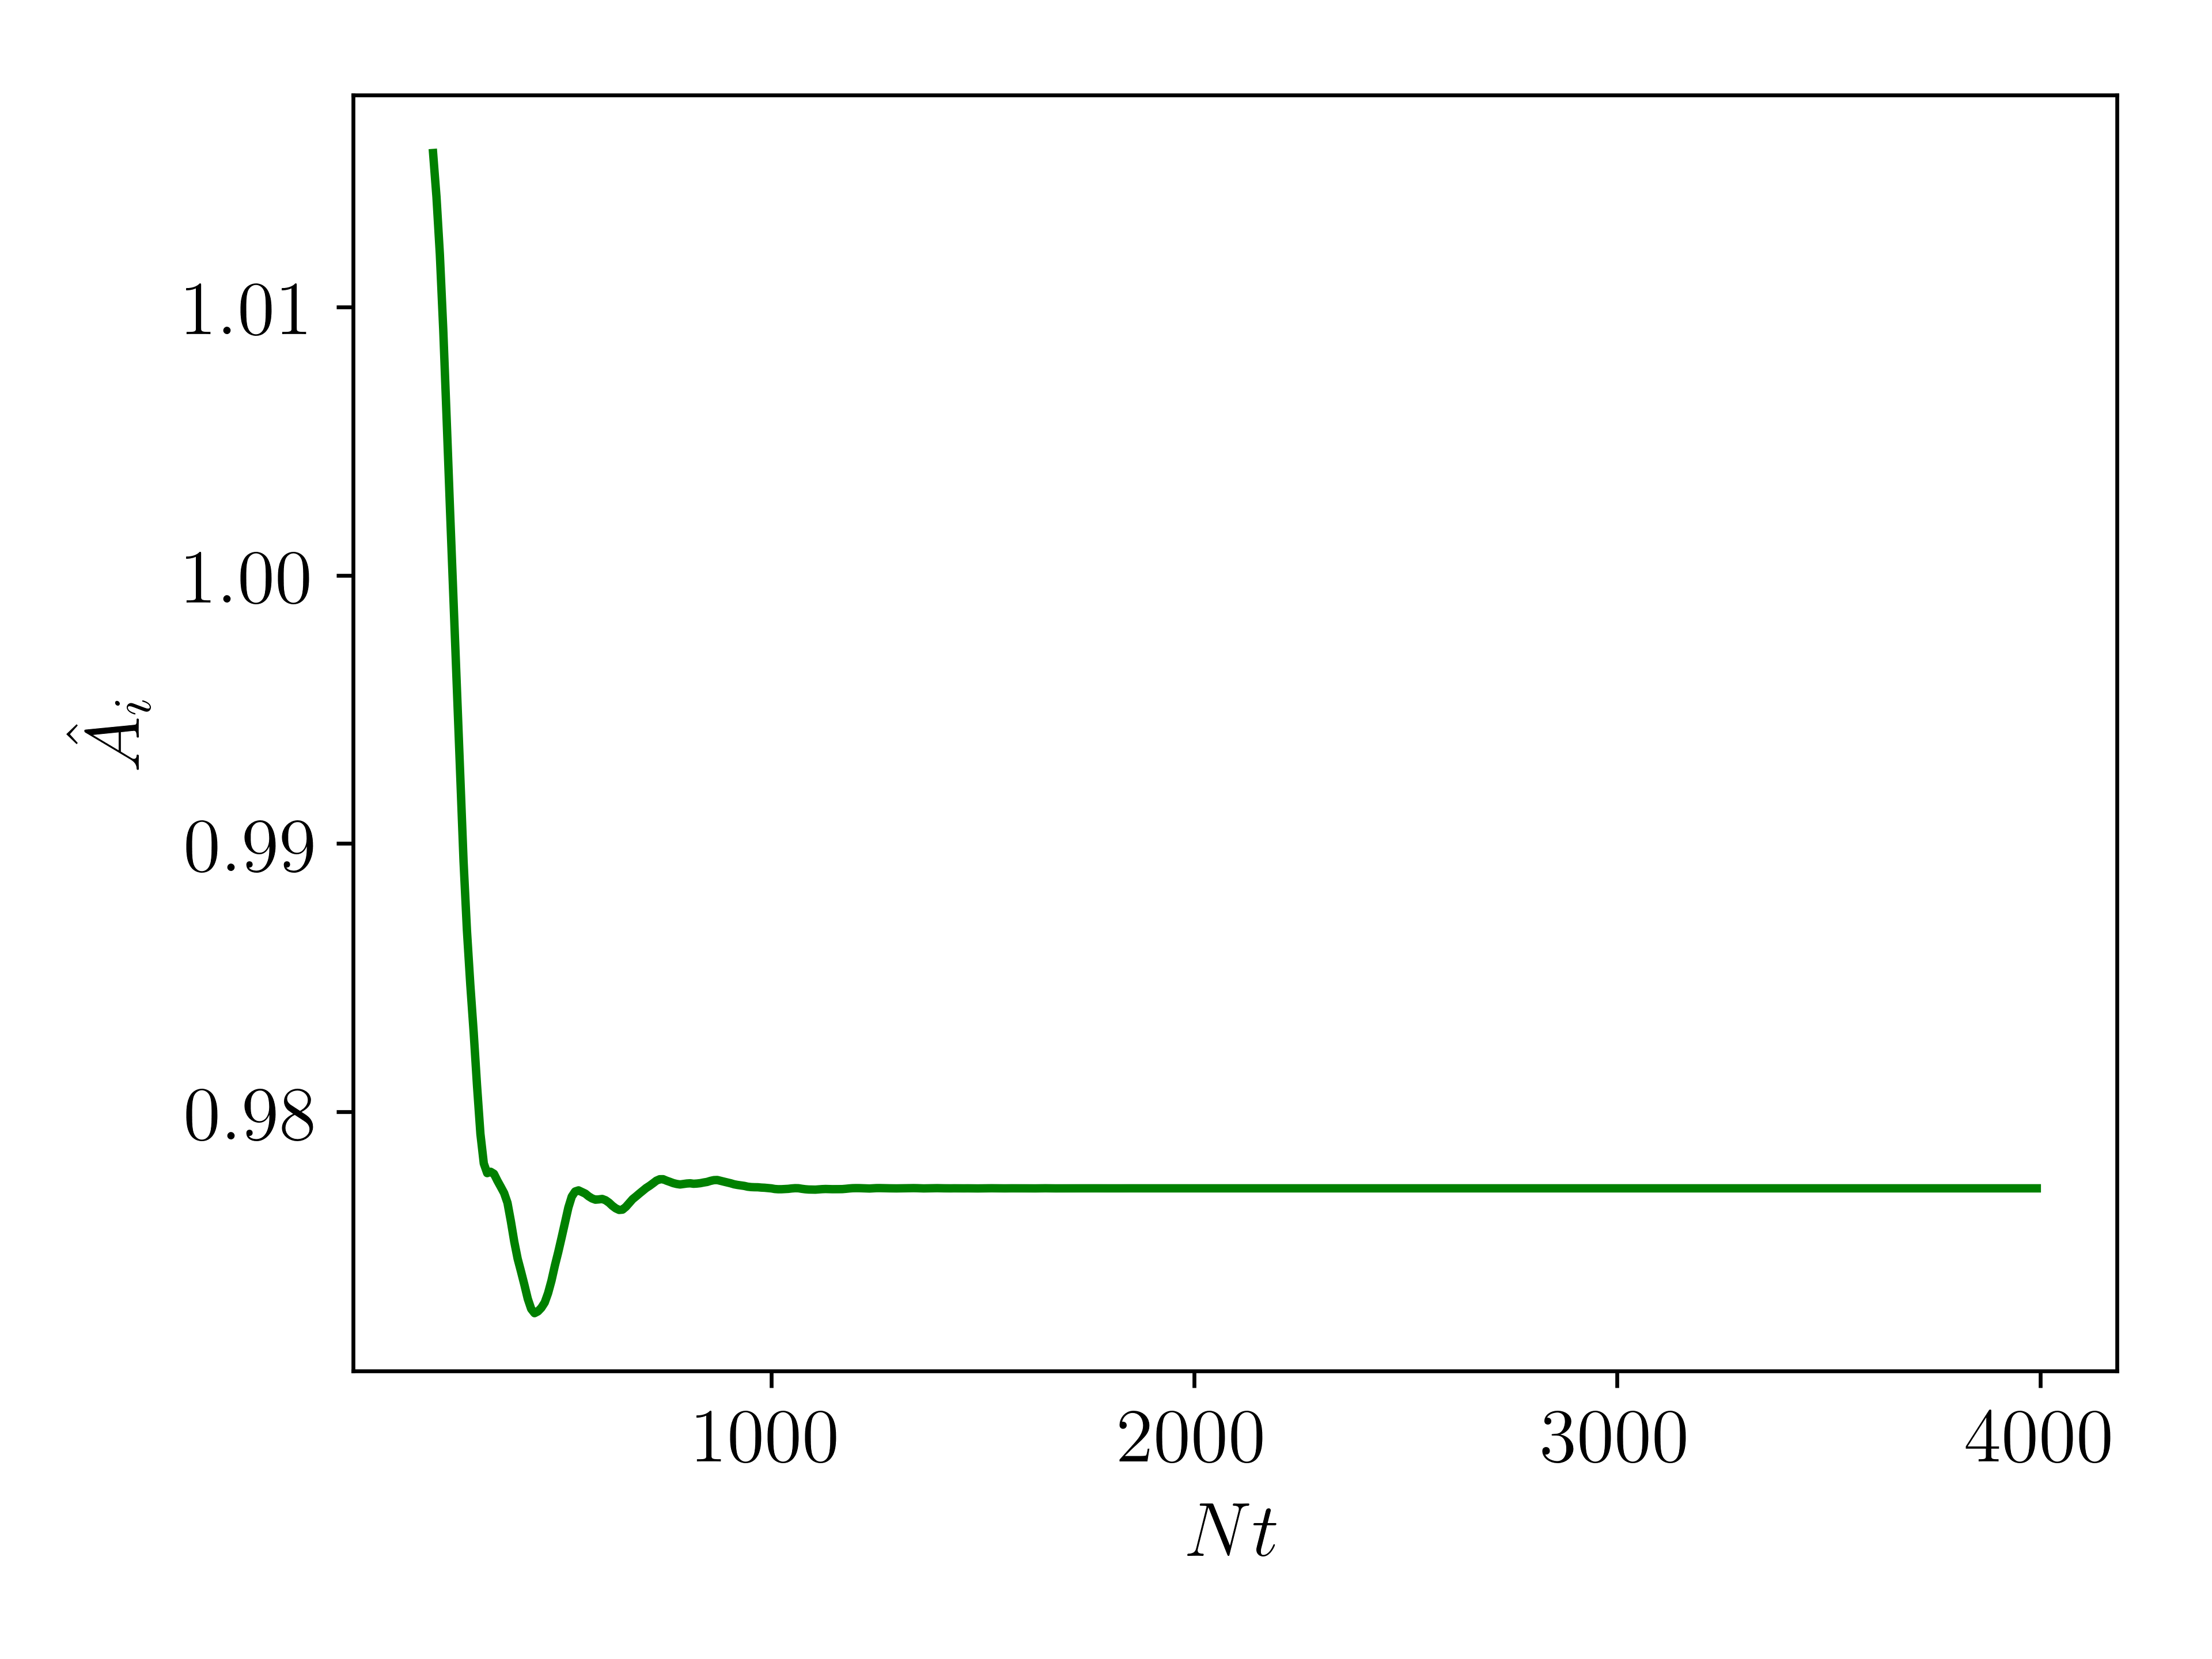
\includegraphics[width=\columnwidth]{plots/lin_amps.png}
    \caption{Amplitude of excited wave over time in weak forcing simulation,
    computed using \autoref{eq:ahat_def}. $\hat{A}_i(t) = 1$ corresponds to
    perfect agreement with the analytical estimate. After an initial transient
    phase, we observe great agreement with \autoref{eq:uz_lin}, and in
    particular $\hat{A}_i(t)$ asymptotes to a constant value, implying continuous
    excitation of identical IGW.}\label{fig:lin_amps}
\end{figure}

The analytical theory also predicts that the horizontal momentmum flux $F(z, t)$
should be spatially flat between the forcing zone where it is generated and the
damping zone where it is dissipated (\autoref{eq:F_def}). We make may a slightly
more accurate estimate of the flux carried in the IGW by directly substituting
$\bm{u}_{al}'$ into \autoref{eq:F_def}. Calling this estimate
\begin{equation}
    F_{al}'(z) \equiv \ev{\overline{\rho} u_{al,x}'u_{al,z}'}_x
\end{equation}
we may then measure the agreement of our simulation with analytical expectation
by computing
\begin{equation}
    \hat{F}(z, t) \equiv \frac{\ev{\rho u_xu_z}_x}
        {F_{al}'}.\label{eq:sbm_def}
\end{equation}
For our weak forcing simulation, $\hat{F}(z) = 1$ is expected between $z_0, z_T$
after initial transients dissipate, and indeed we observe agreement with this in
\autoref{fig:lin_fluxes}.
\begin{figure}
    \centering
    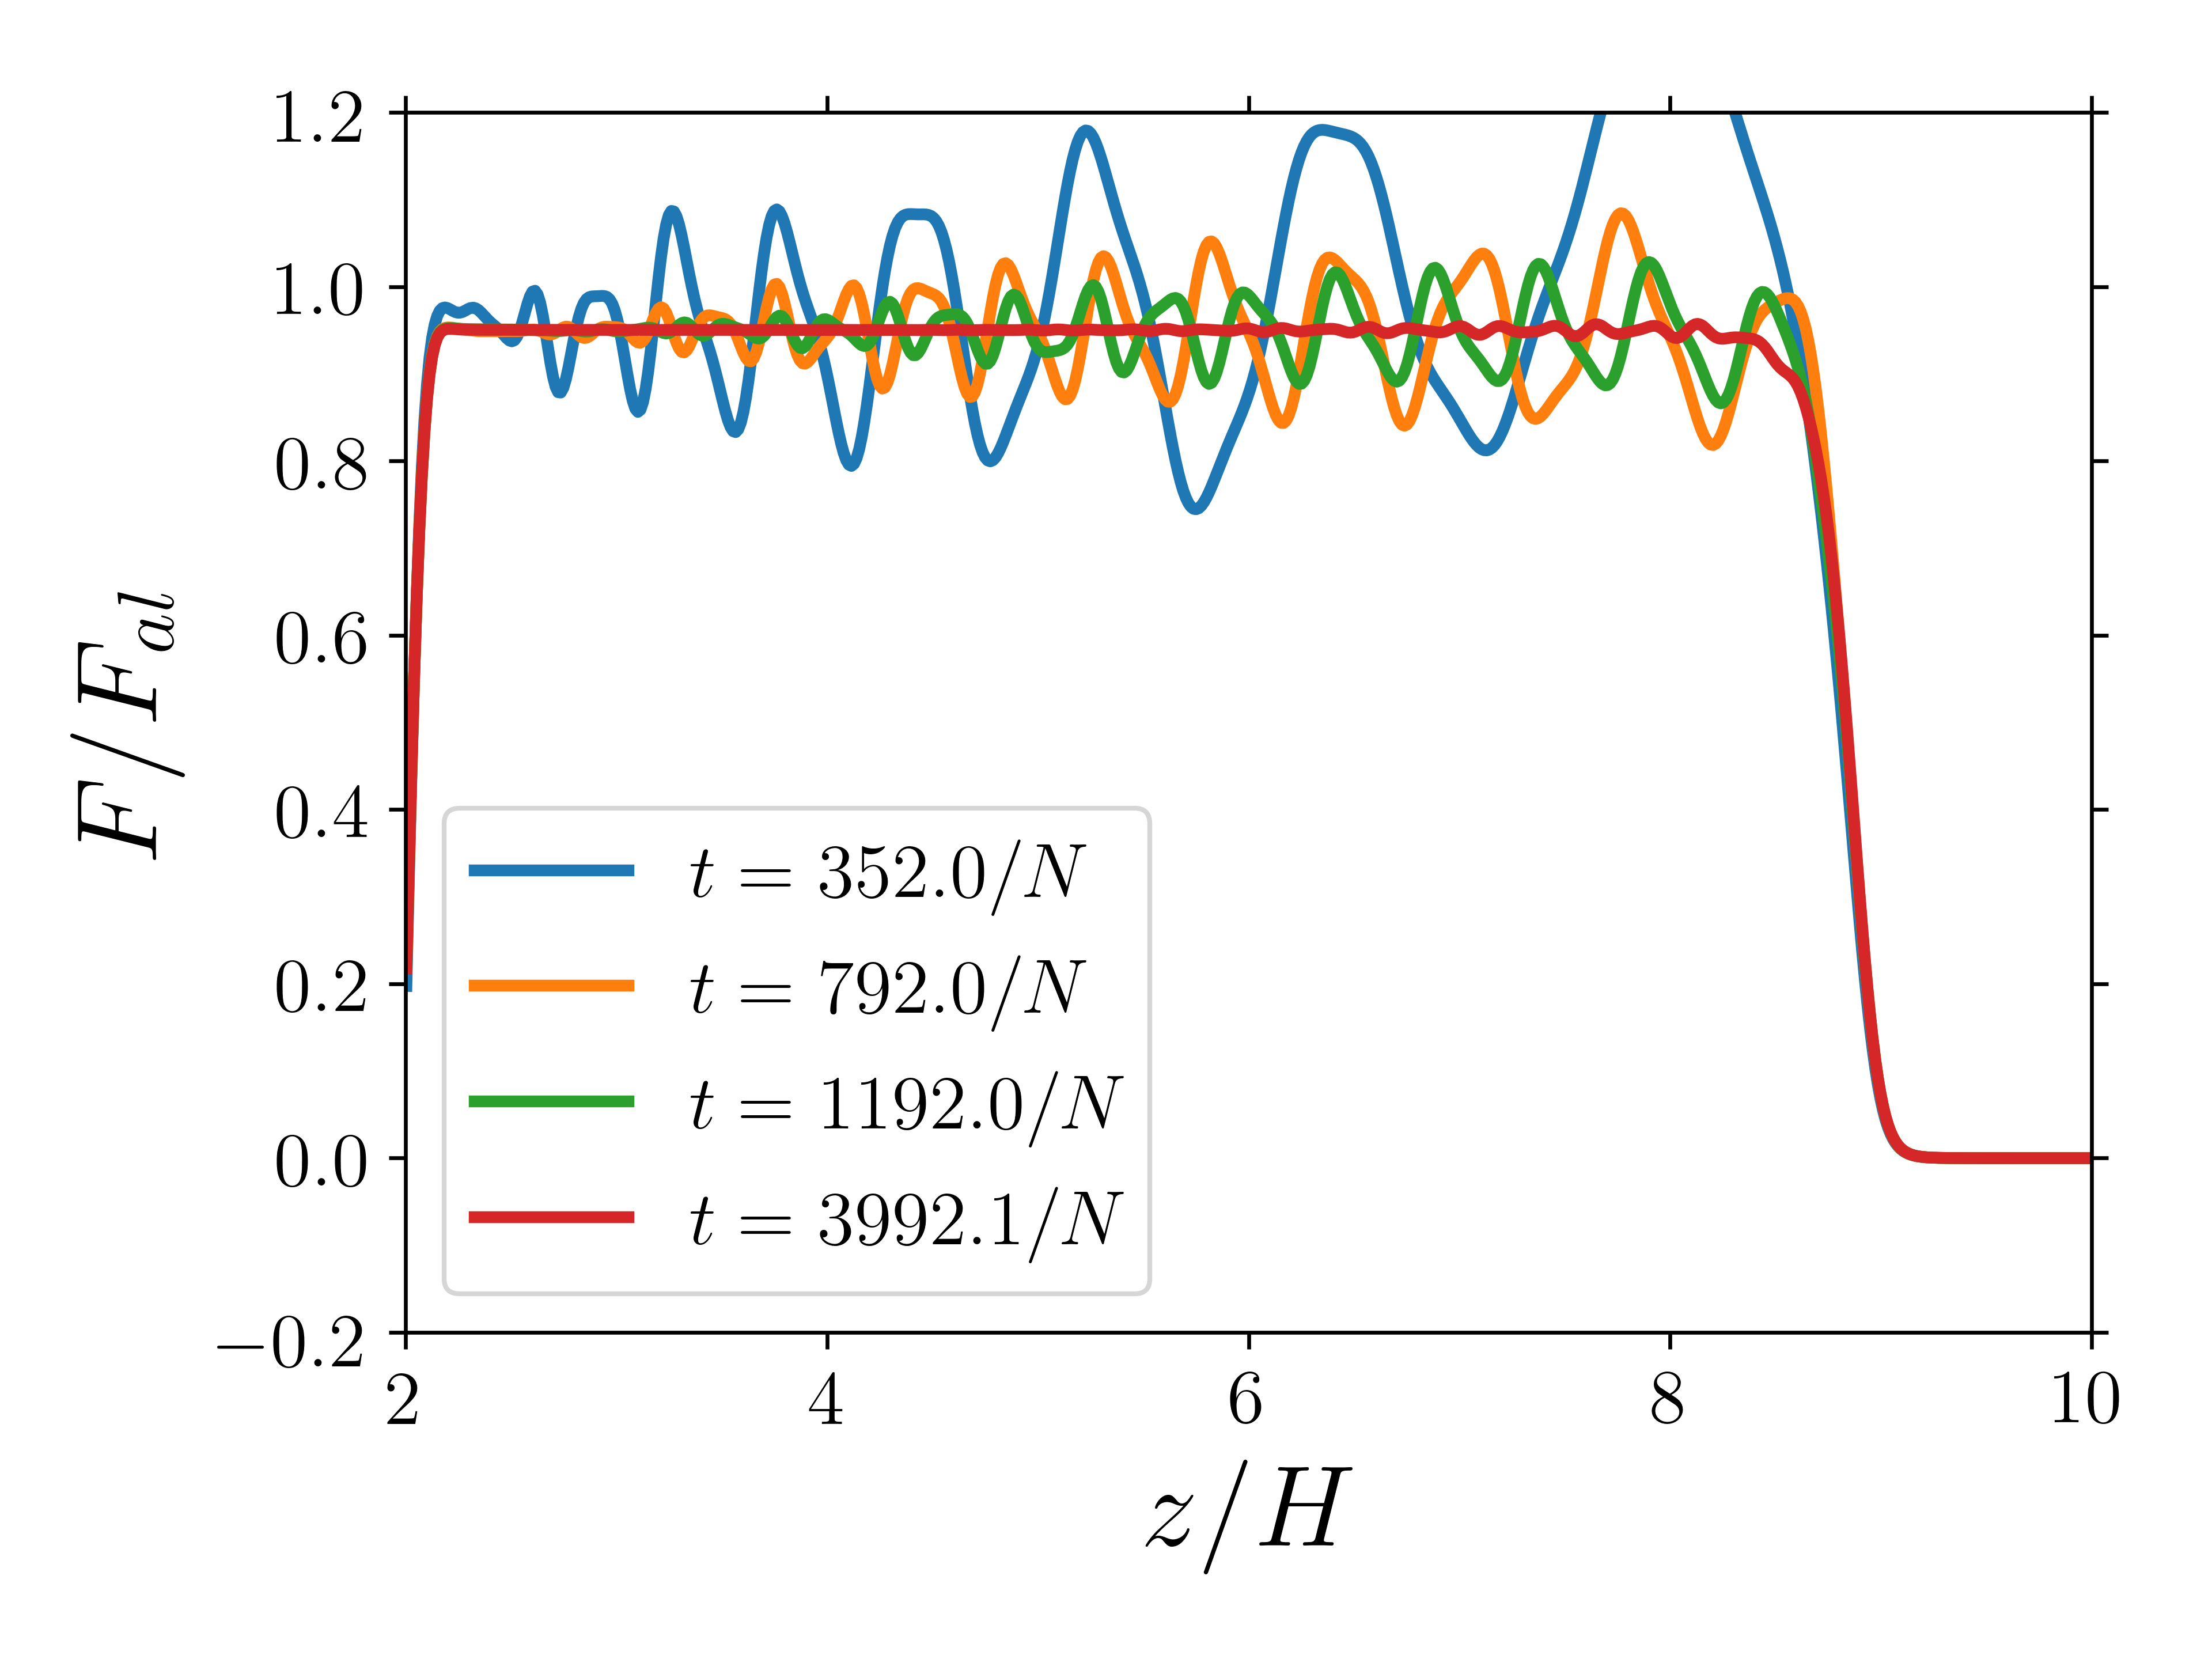
\includegraphics[width=\columnwidth]{plots/lin_fluxes.png}
    \caption{\autoref{eq:sbm_def} as a function of $z$ at select times $t$. As
    initial transients die out, $\hat{F}(z, t) = 1$ to very good agreement above
    the forcing zone $z > z_0 = 2H$ and below the damping zone $z \lesssim z_T =
    9.5H$. The flux excited in the forcing zone is transported without loss to
    the top of the domain, where it is dissipated by the damping layer (see
    \autoref{ss:damping}) without reflection.}\label{fig:lin_fluxes}
\end{figure}

\section{Internal Gravity Waves: Nonlinear Simulation}\label{s:sim}

% times on fluxes.png are 054, 086, 153

To perform simulations of wave breaking phenomena, we use the same values as
\autoref{ss:numerics} except for $C, \nu$. In particular, we choose $C$ such
that $\at{\xi_z k_z}_{z_0} = 0.1$ in the forcing zone, which implies $\xi_z k_z
$ exceeds $1$ before $z_T$ the upper damping zone. The dissipation parameter
$\nu$ was varied across the various simulations. To quantify $\nu$, we define
dimensionless Reynolds number
\begin{equation}
    \mathrm{Re}  \equiv \frac{\omega}{\nu k_{z}^2}. \label{eq:re_def}
\end{equation}
A table of our simulation viscosities can be found in \autoref{tab:params}.
\begin{table}
    \centering
    \begin{tabular}{l c c c}
        Resolution & $\mathrm{Re}$\\\bottomrule
        $1024 \times 4096$ & $2048$\\
        $768 \times 3072$ & $1024$\\
        $512 \times 2048$ & $512$\\
        $256 \times 1024$ & $341$\\
        $256 \times 1024$ & $205$\\
        $256 \times 1024$ & $146$\\
    \end{tabular}
    \caption{Table of simulation resolutions. Note that $\mathrm{Re}$ is defined
    as in \autoref{eq:re_def}.}\label{tab:params}
\end{table}

\subsection{Numerical Simulation Results}\label{ss:nl_ns}

A full video of our higher-resolution run at $N_x = 768, N_z = 3072,
\mathrm{Re} = 1024$ is available
online\footnote{http://www.princeton.edu/~lecoanet/data/breaking\_wave.mov}. We
take this to be our fiducial simulation for the remainder of this paper, though
other simulations show qualitatively identical behavior. Snapshots of the
velocity field $\bm{u}$ at select times can be found in \autoref{fig:snapshots}.
% convert yubo_000054.png -crop 2000x2000+150+250 out.png
\begin{figure*}
    \subfloat[$t=413.4$ At early times, the flow resembles a linear IGW lower in
    the simulation domain but breaks down into smaller-scale features at higher
    $z$. Some characteristic swirling motion can be seen in both $u_x, u_z$,
    highly suggestive of Kelvin-Helmholtz instabilities.]{
    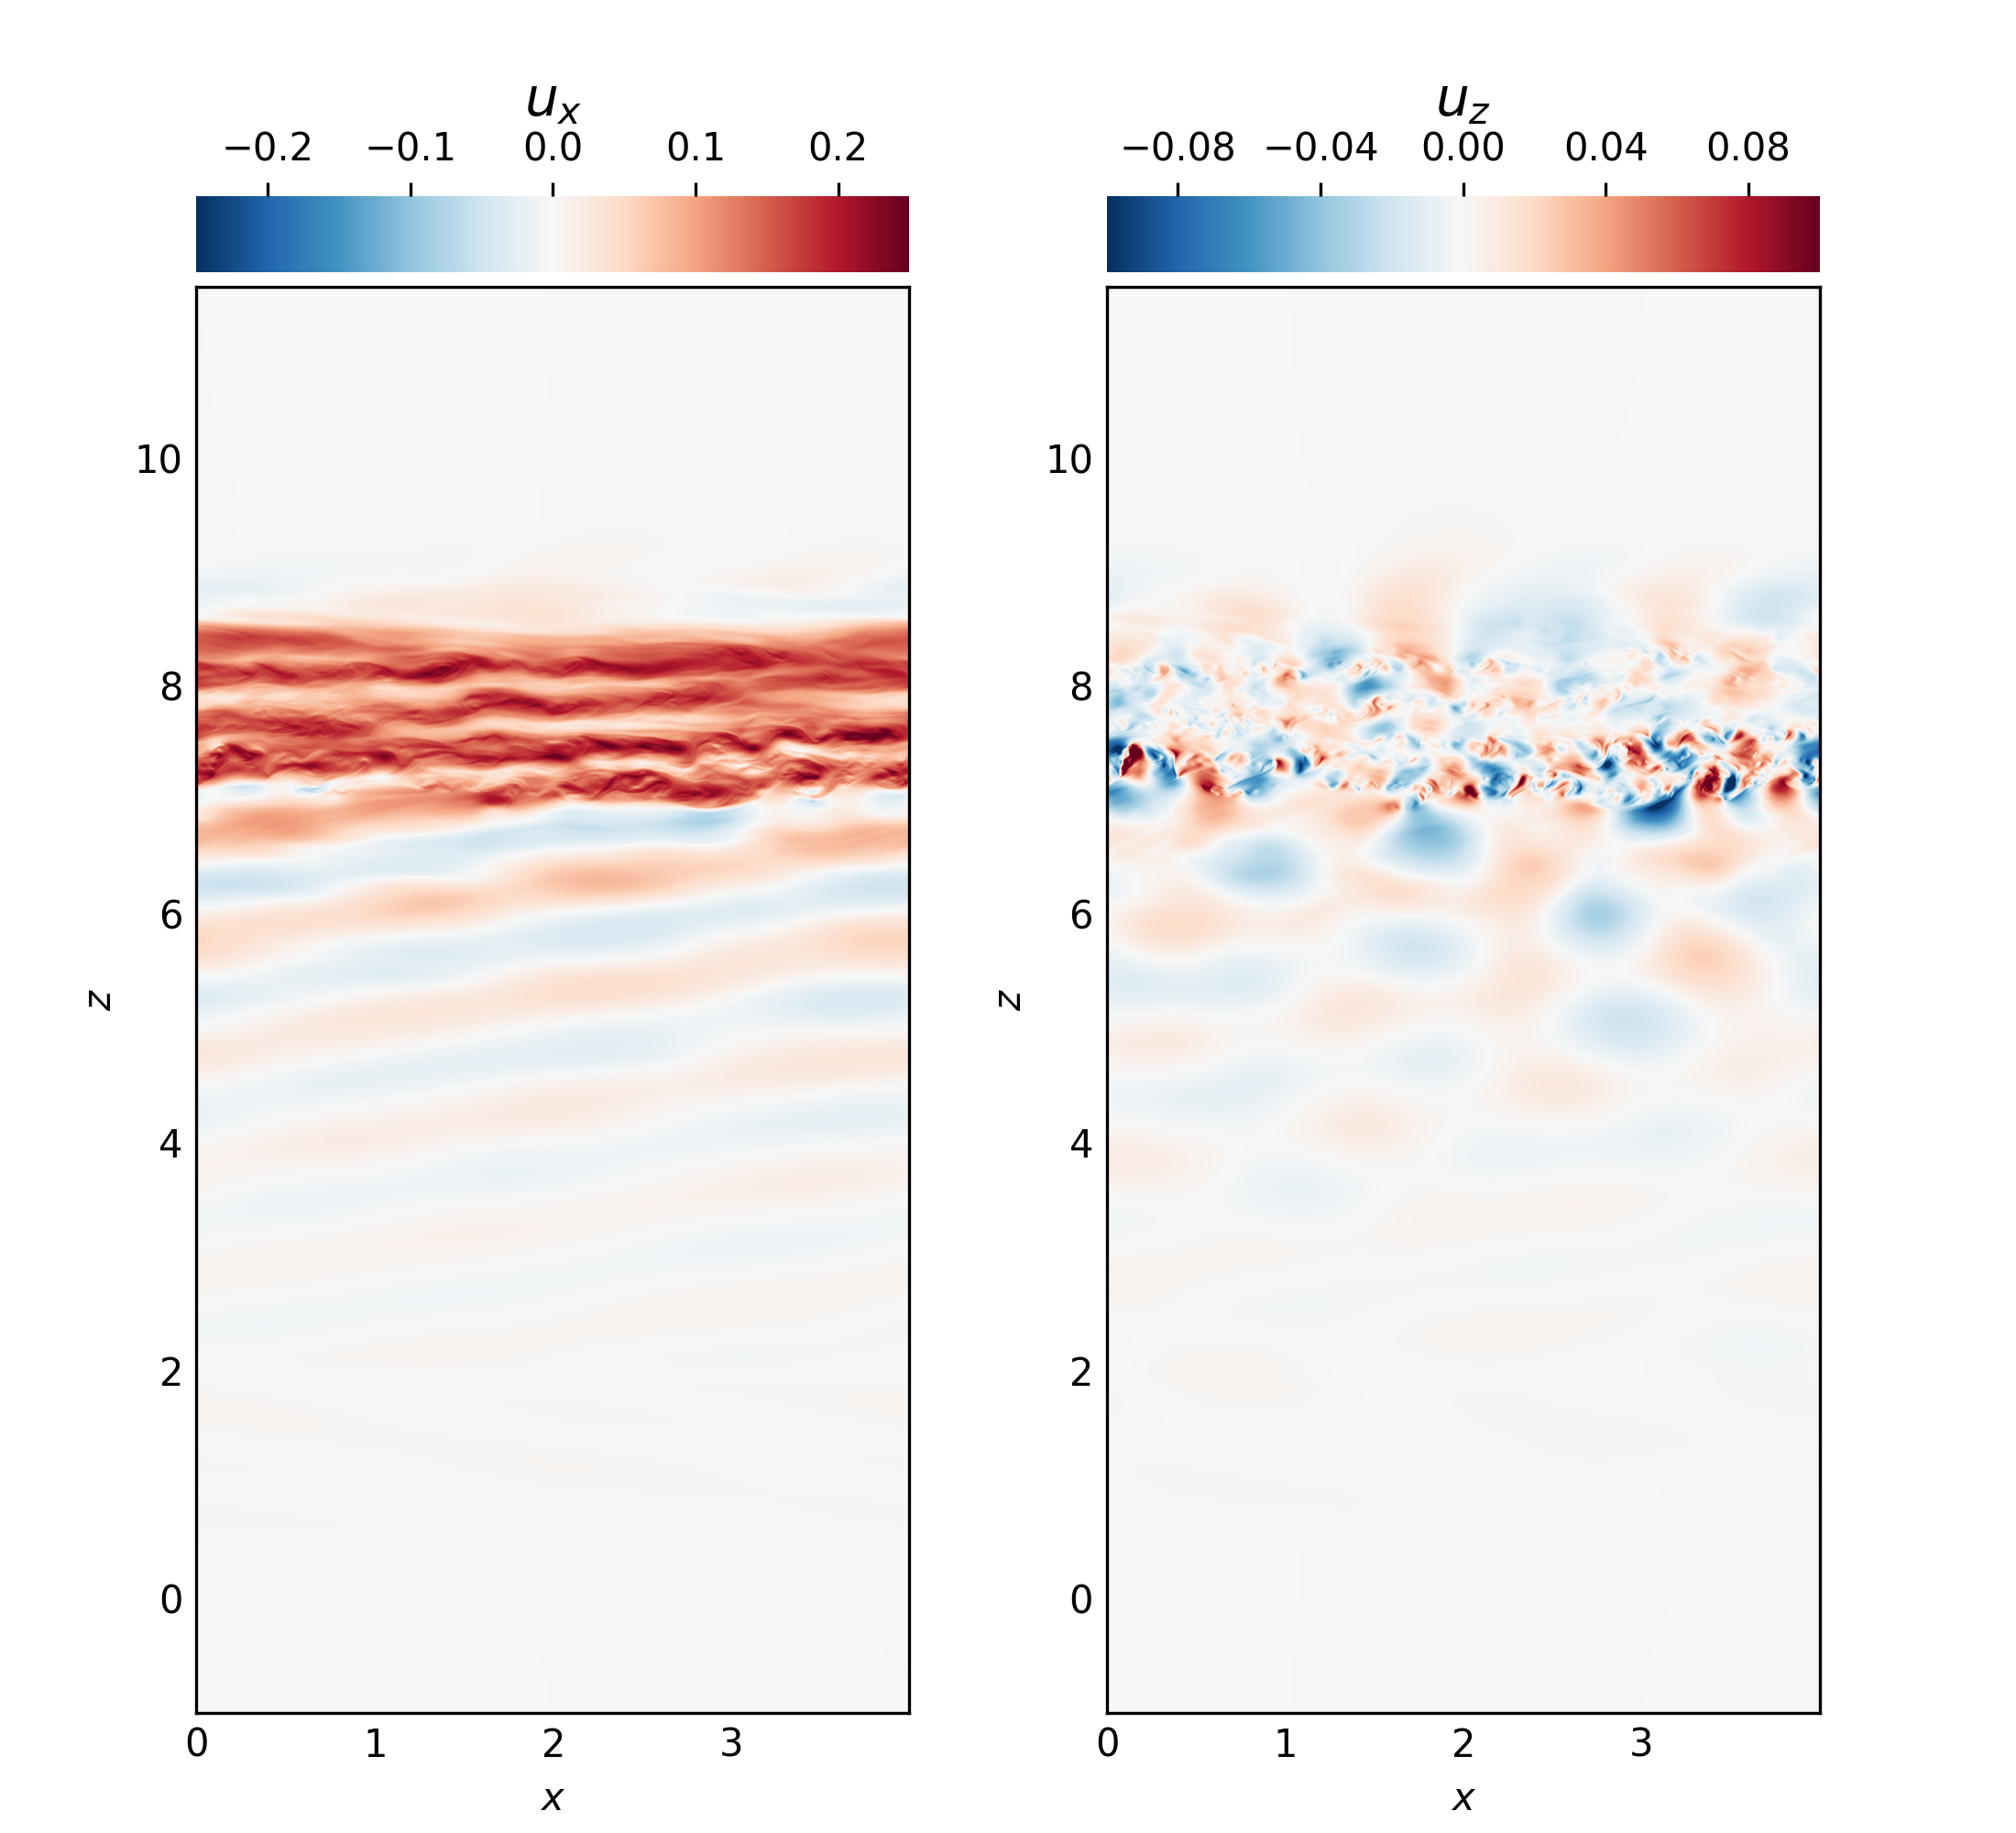
\includegraphics[width=0.45\textwidth]{plots/yubo_000054.png}}\hfil
    %
    \subfloat[$t=658.5$ At a slightly later time, the mean flow in $u_x$ has
    become much more prominent and the critical layer $z_c$ has become much more
    definite. Small-scale fluctuations are still present in $u_z$ albeit at
    smaller amplitudes due to being in a denser region of the fluid.]{
    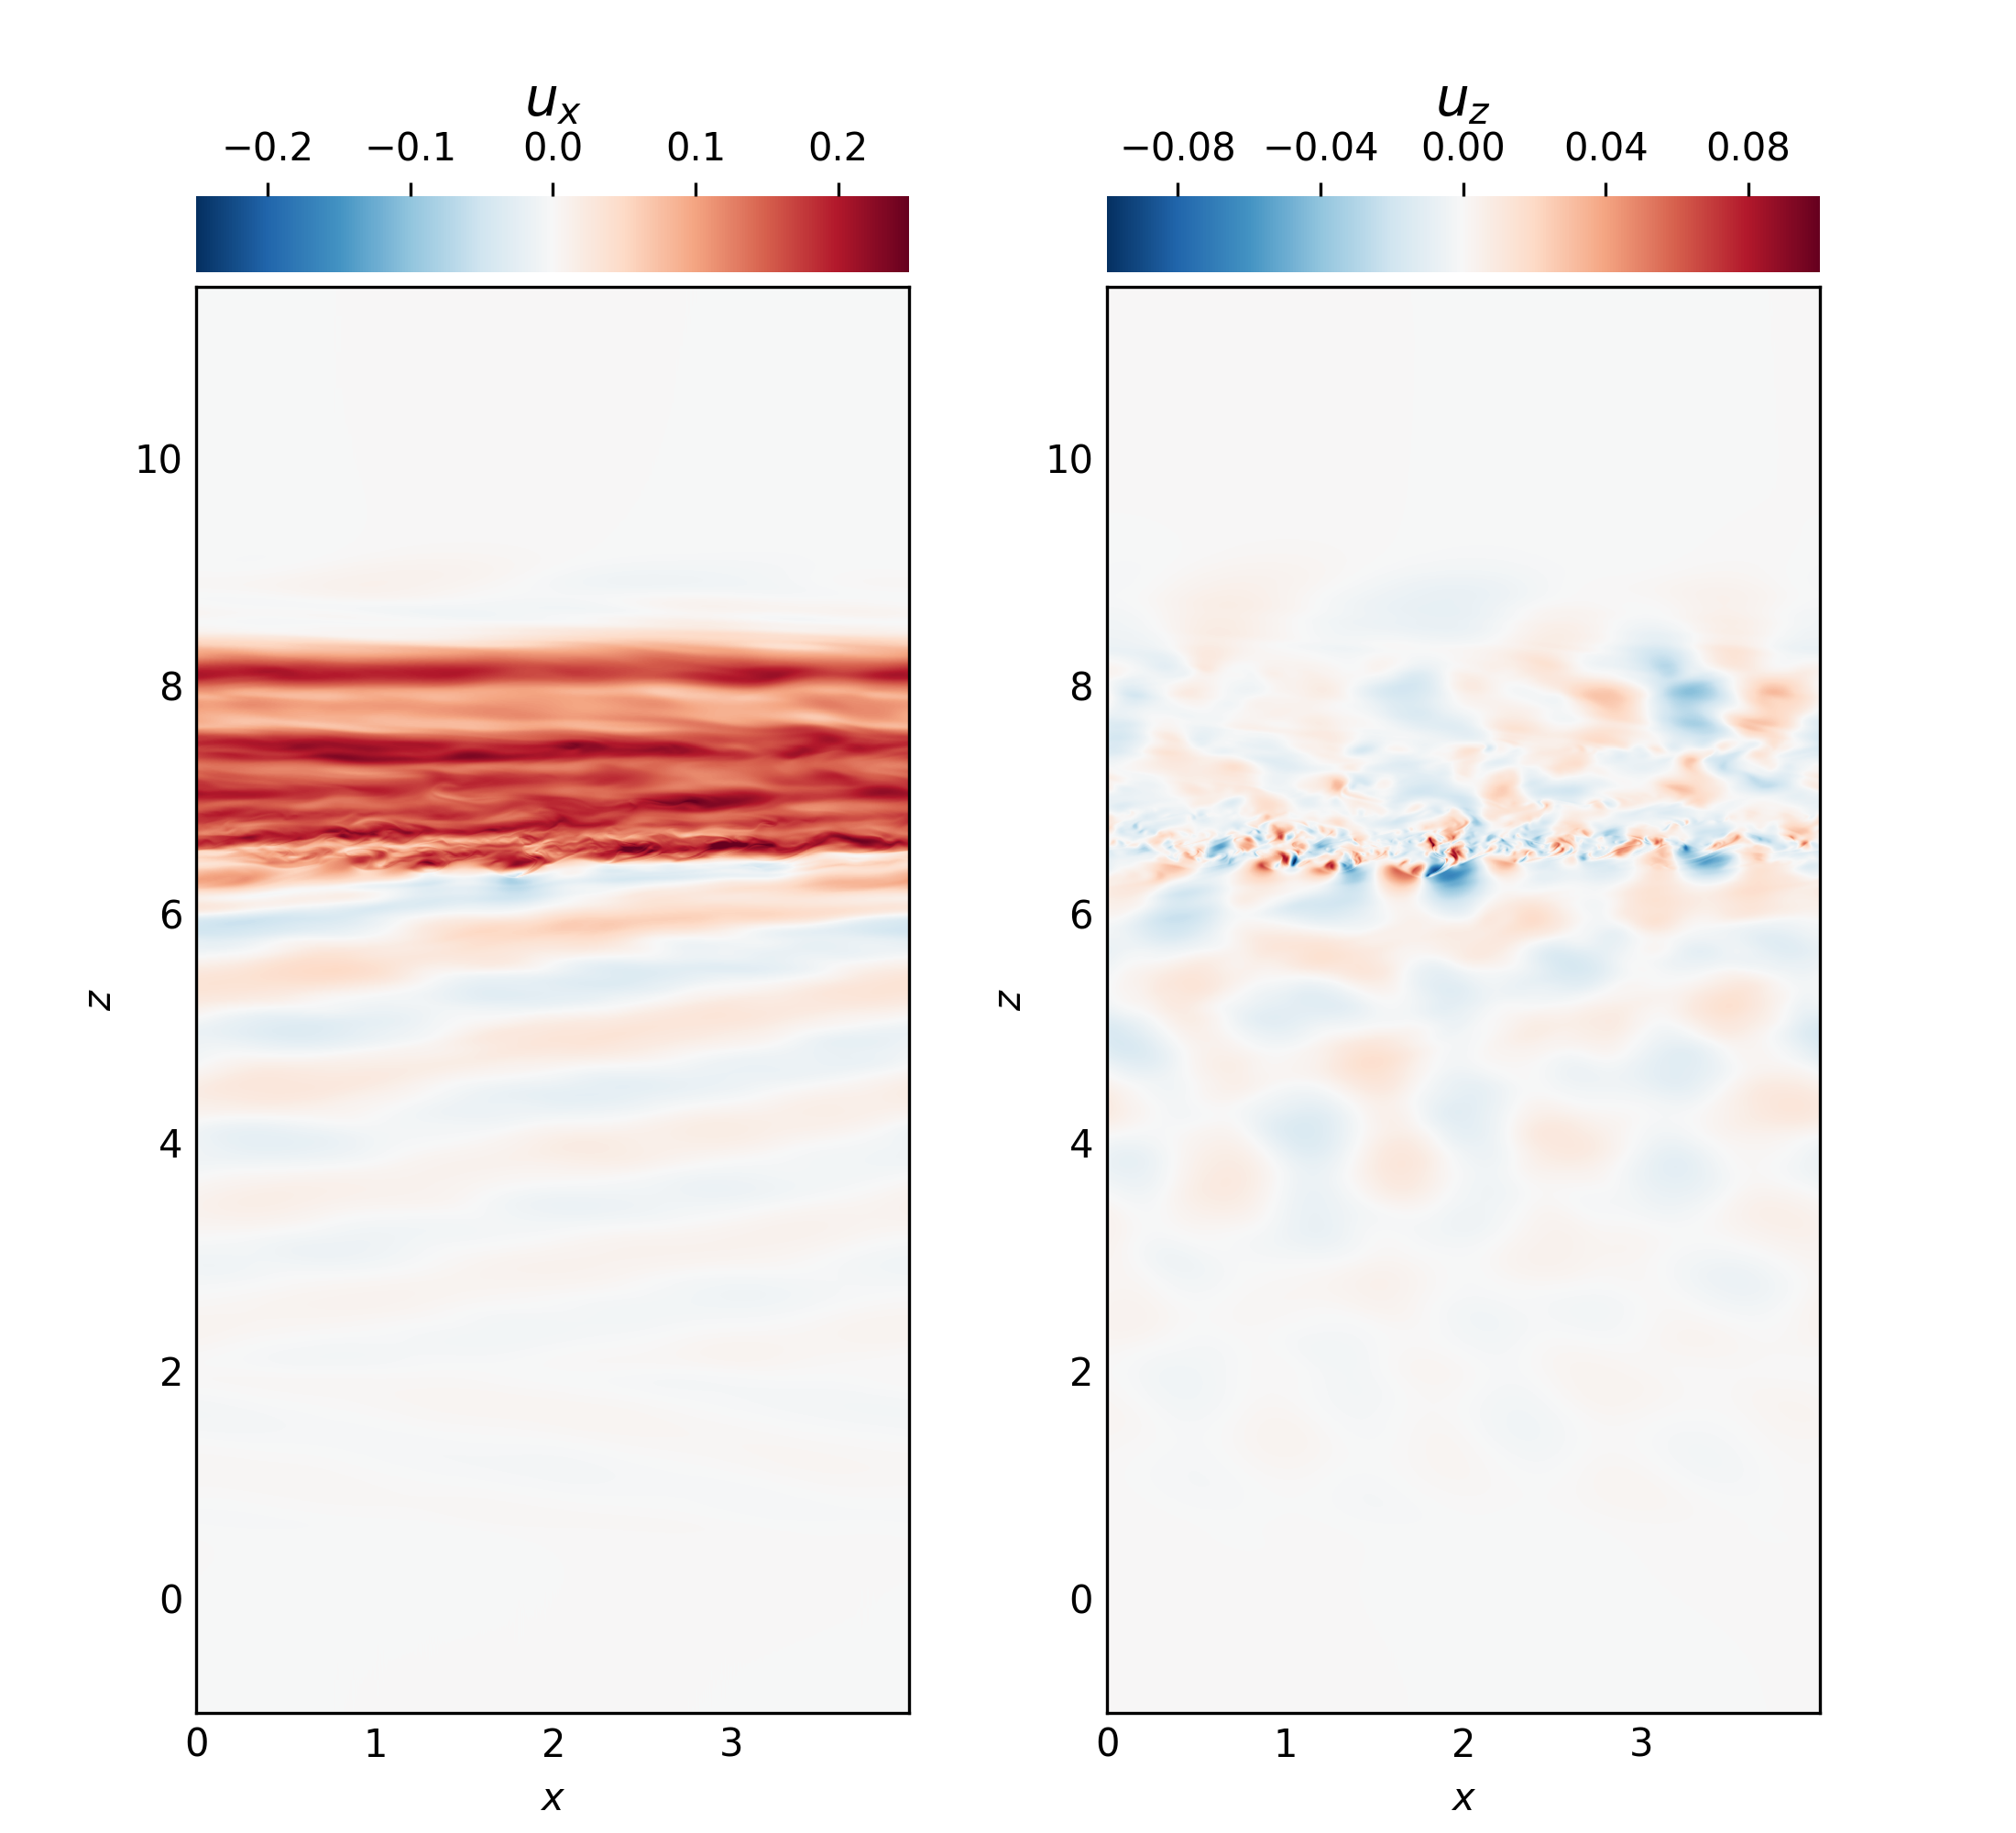
\includegraphics[width=0.45\textwidth]{plots/yubo_000086.png}}

    \subfloat[$t=1171.4$ The critical layer transition is now extremely sharp,
    and small swirls of limited vertical extent at the location of the critical
    layer in $u_z$ suggest that the Kelvin-Helmholtz instability is responsible
    for regulating the minimum width of this transition, a hypothesis explored
    in \autoref{ss:khi}.]{
    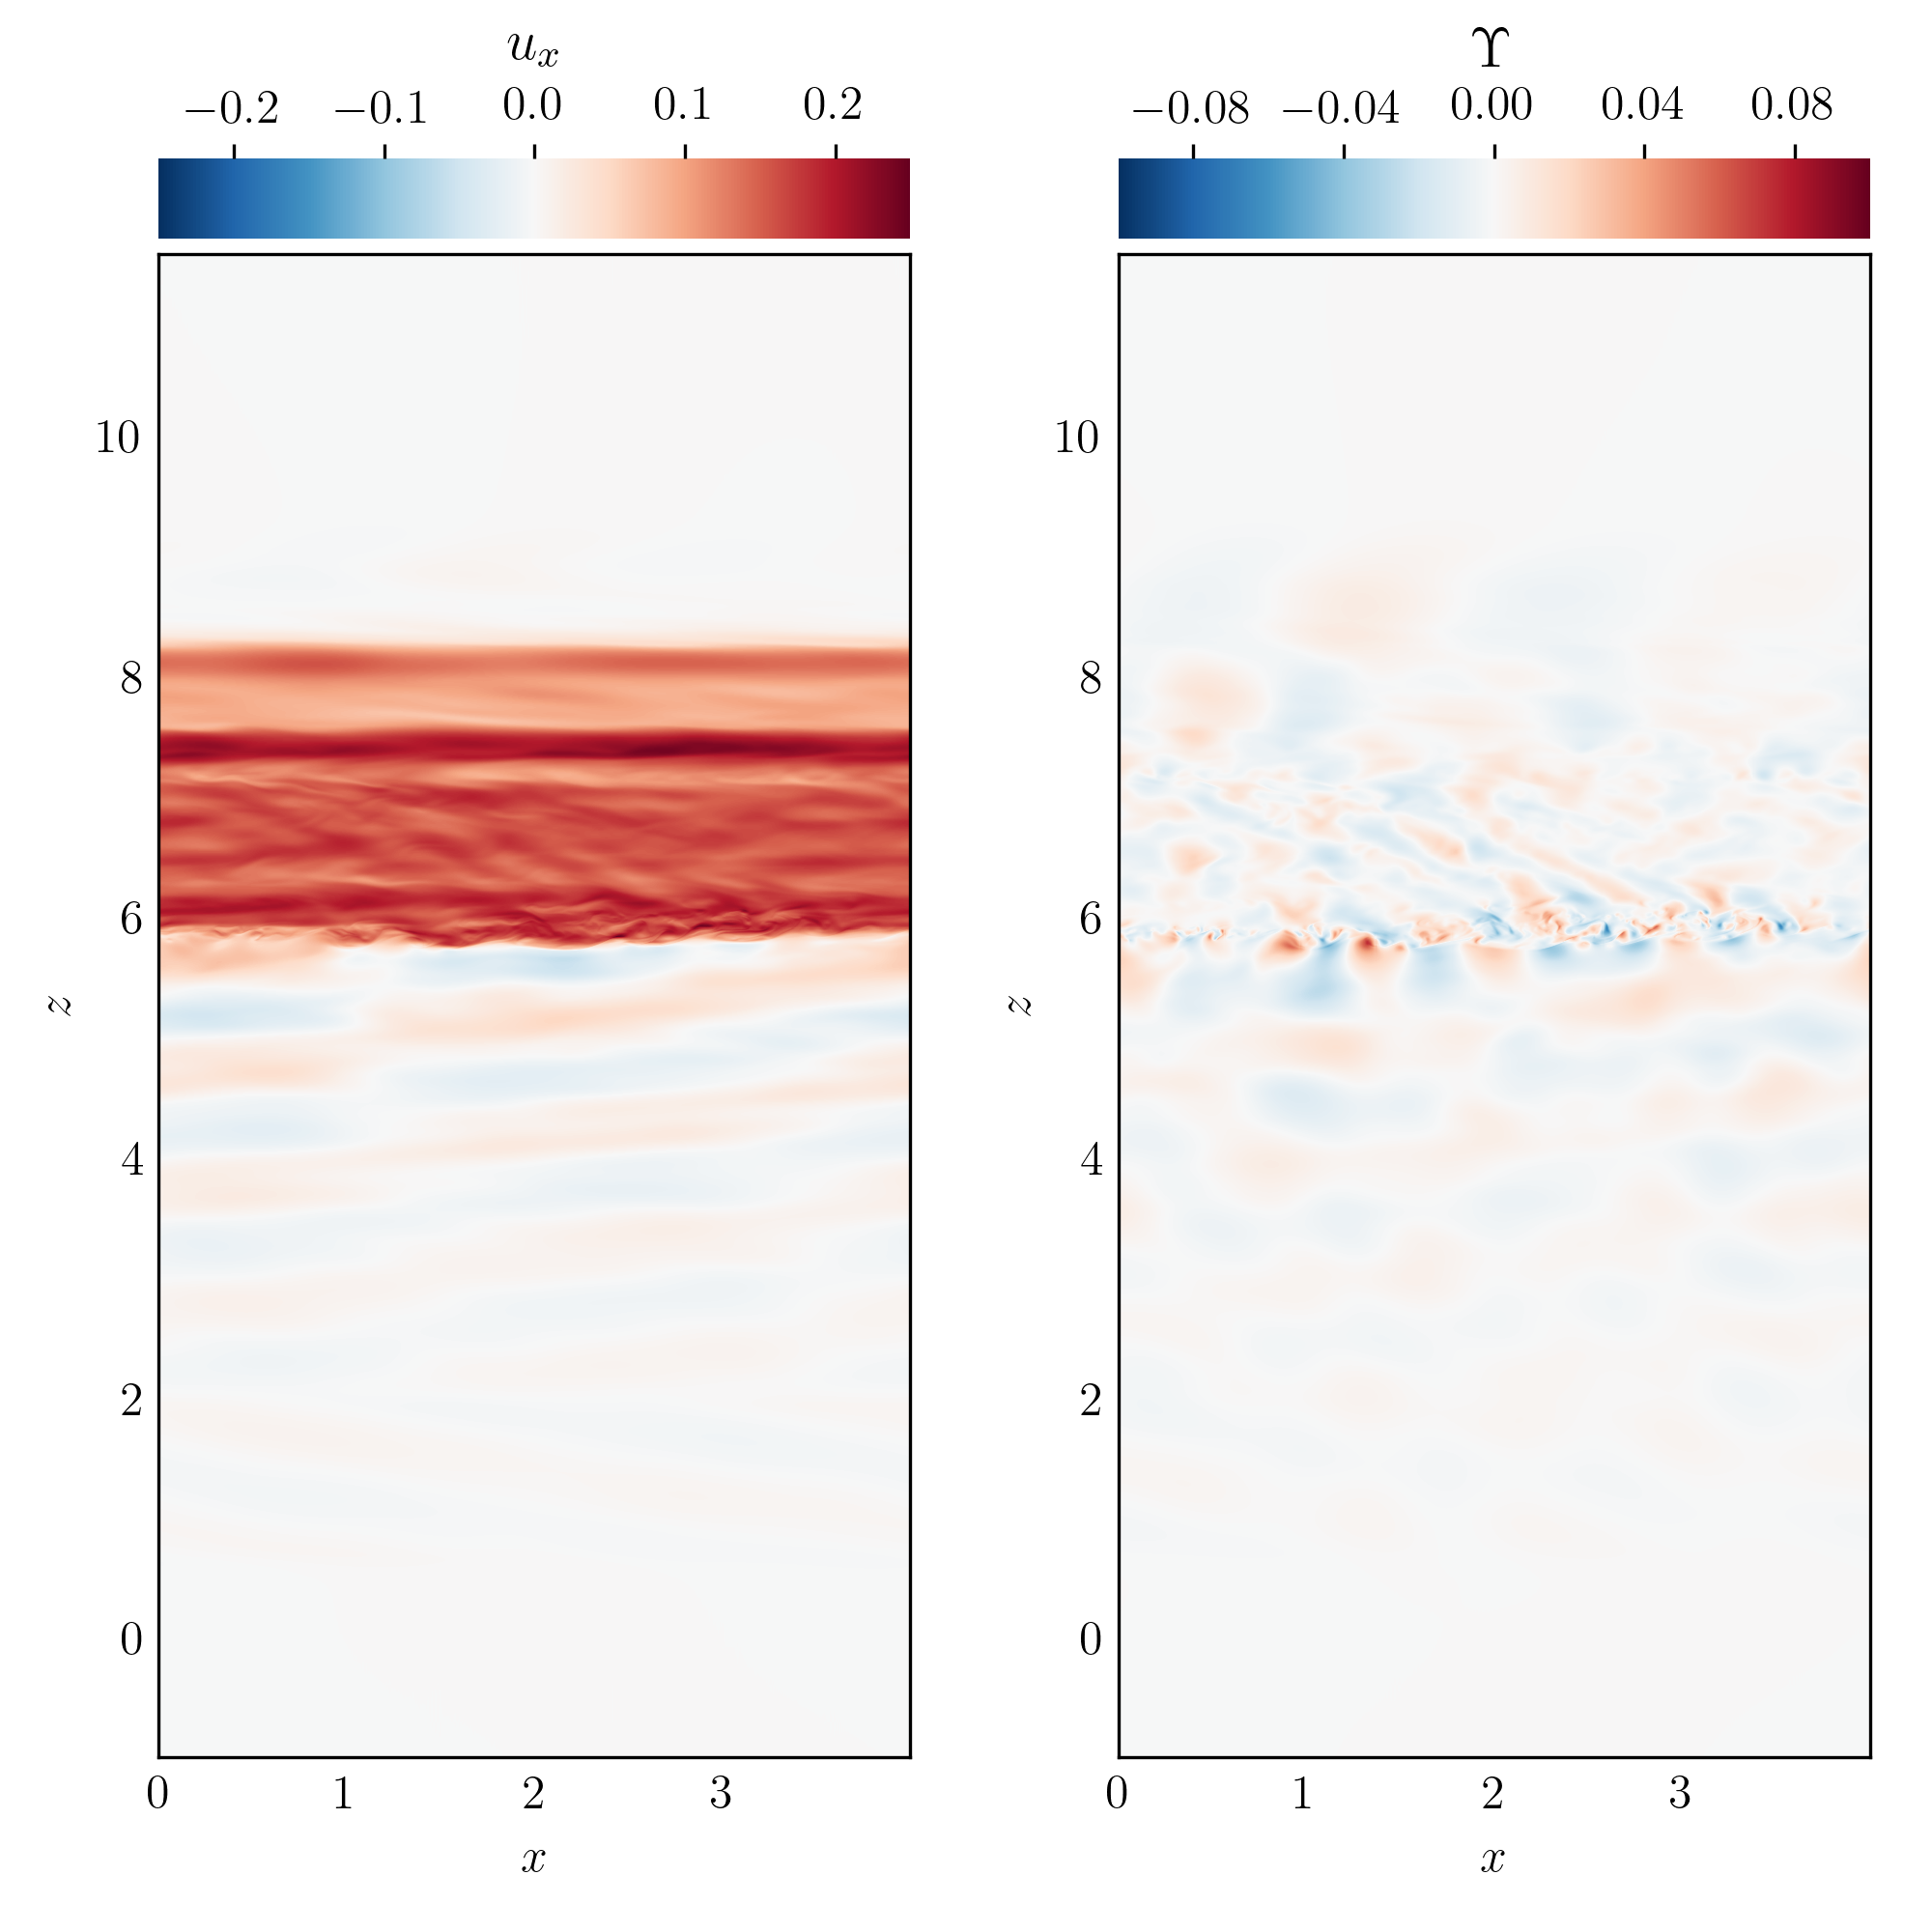
\includegraphics[width=0.45\textwidth]{plots/yubo_000153.png}}\hfil
    %
    \subfloat[$t=3437.8$ The end of the simulation shows very few significant
    qualitative differences from the previous snapshot, suggesting that the
    latter half of our simulation is temporally converged.]{
    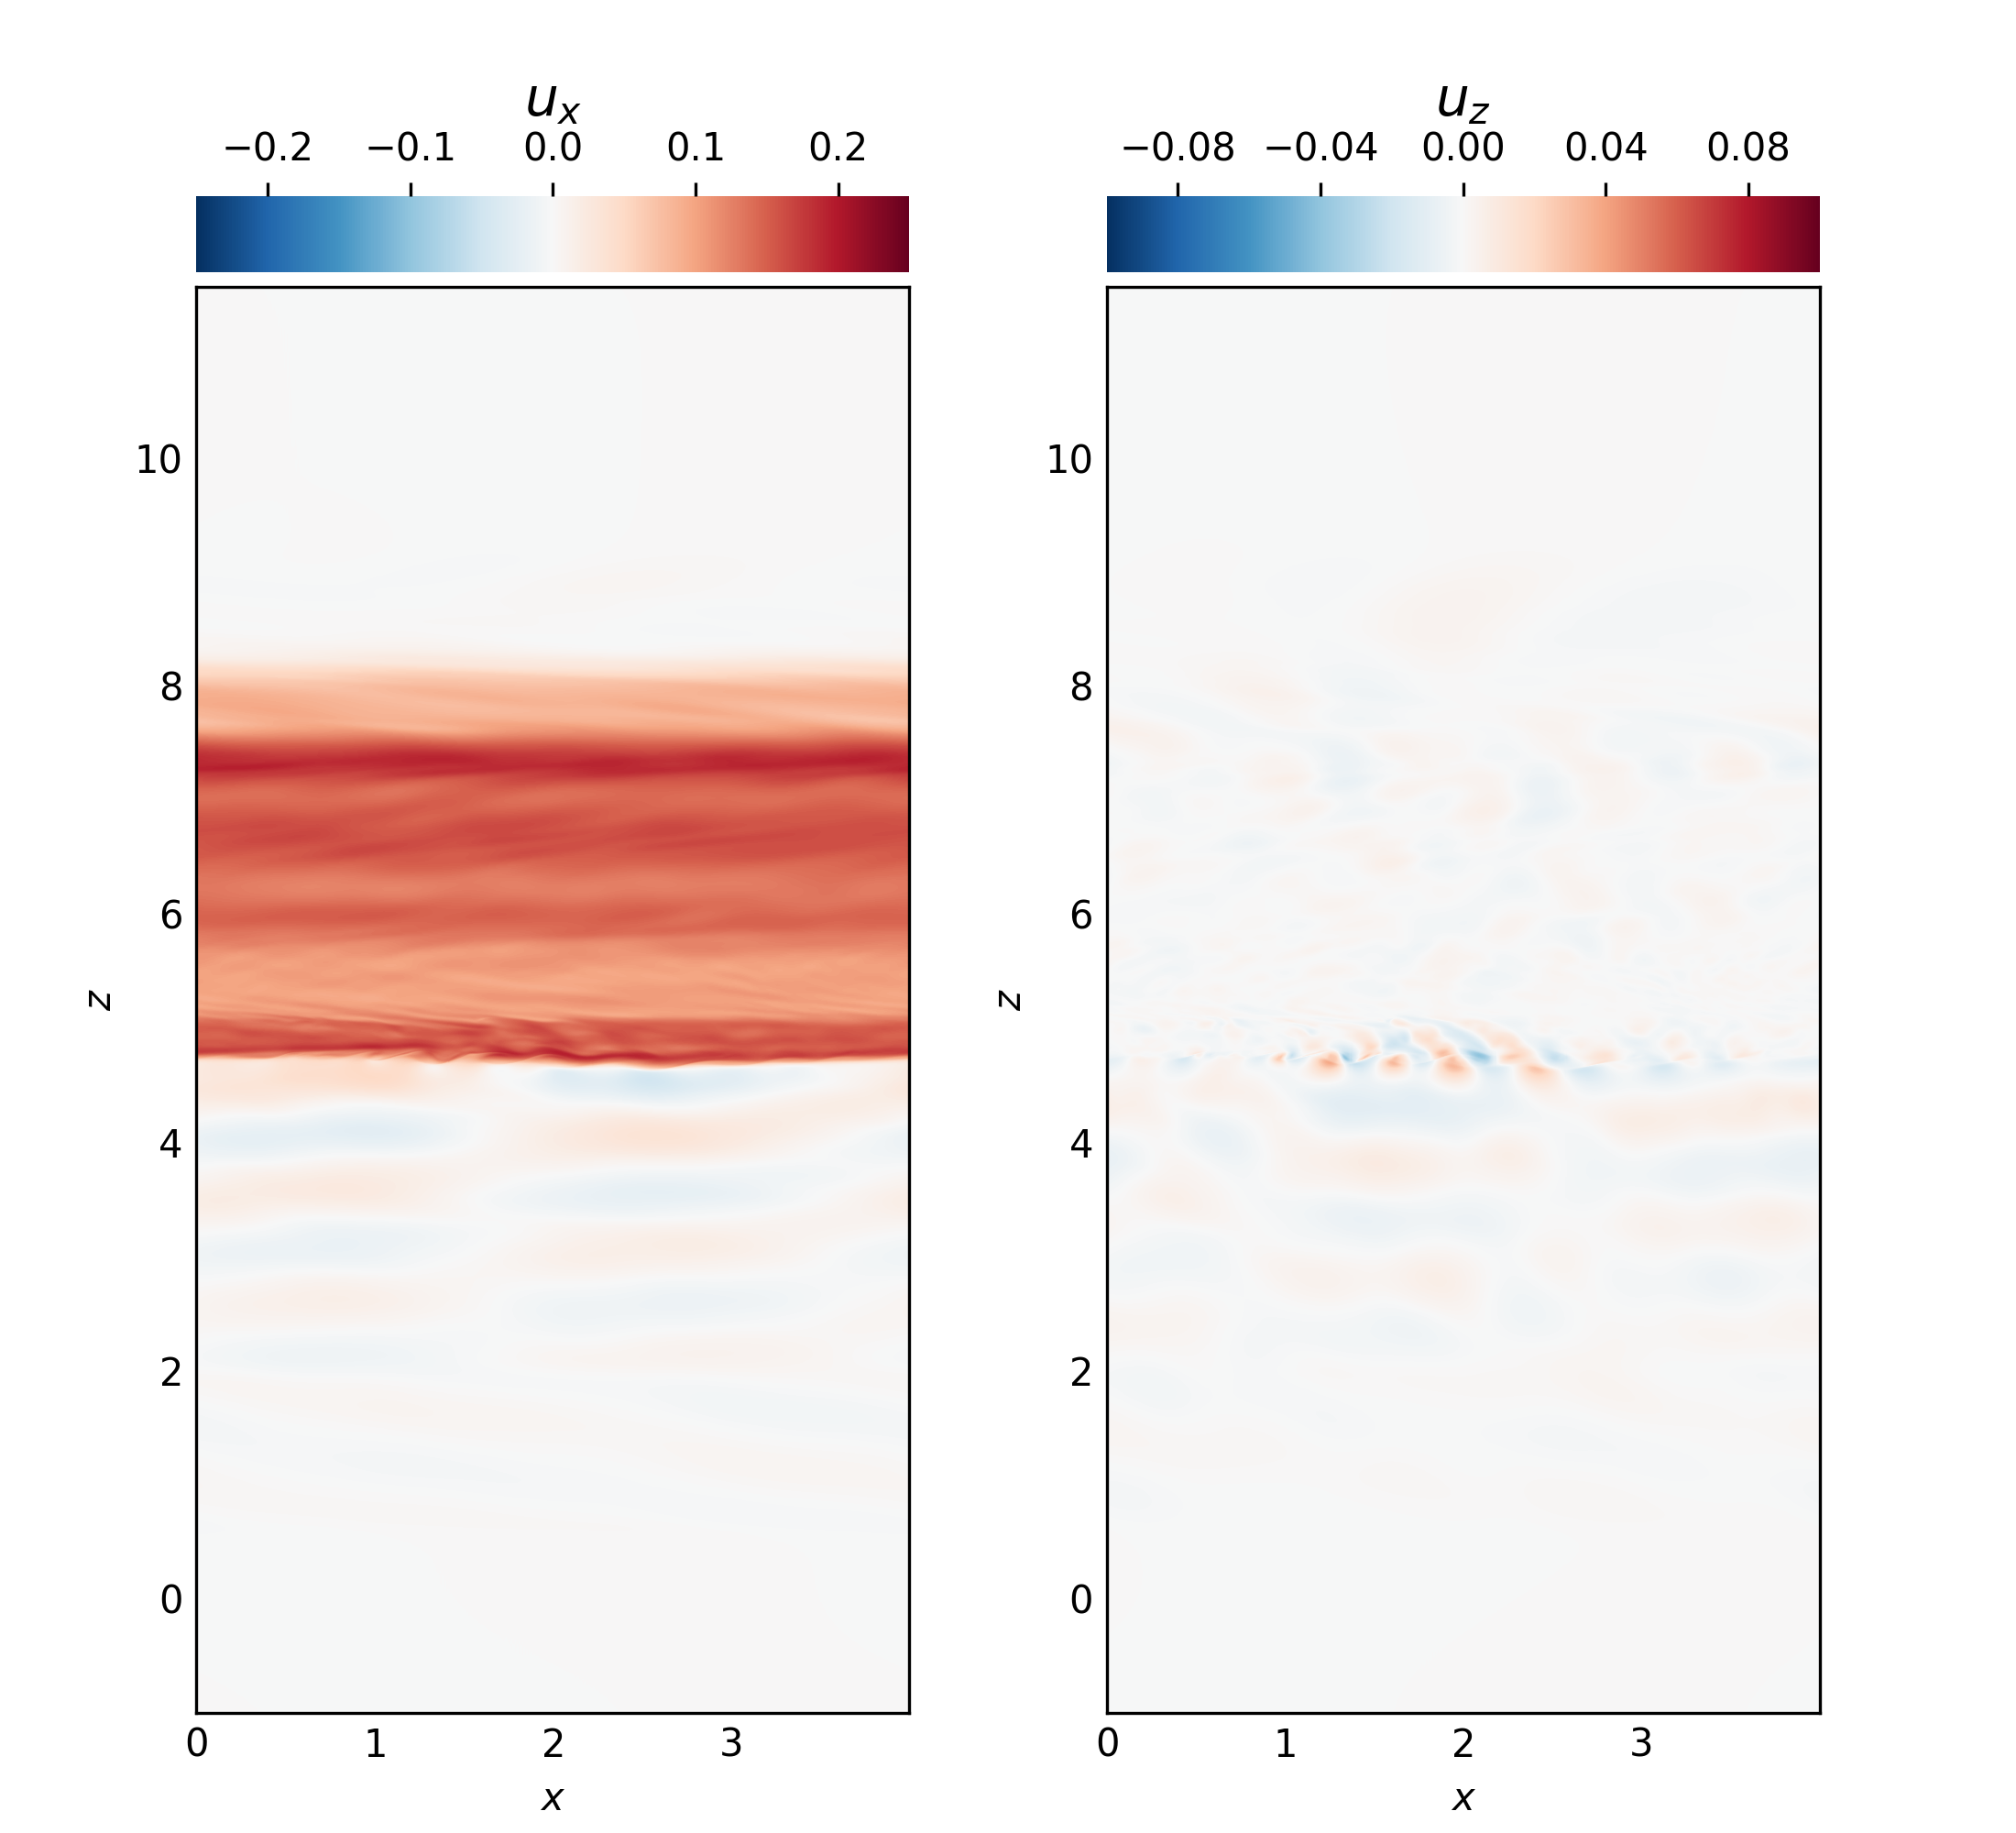
\includegraphics[width=0.45\textwidth]{plots/yubo_000451.png}}

    \caption{Snapshots of $u_x, u_z$ in the fiducial simulation illustrating
    distinct phases of the evolution of the flow. Note that $\overline{U}_c
    \approx 0.16$ for the parameters used.}\label{fig:snapshots}
\end{figure*}

Slices of
$\overline{U}, \hat{F}$ across $z$ at various times $t$ are shown in
\autoref{fig:nl_fluxes}. While the behavior of $\overline{U}$ seems to conform
qualitatively with the predictions of \autoref{ss:crit_layer}, the behavior of
$\hat{F}$ exhibits two salient features: (i) the incident flux seems to
fluctuate greatly with time, and (ii) there seems to be a small transmitted
feature at many of the later times. We will discuss further these features in
\autoref{ss:reflectivity}, after first analyzing the propagation of the critical
layer.
\begin{figure}
    \centering
    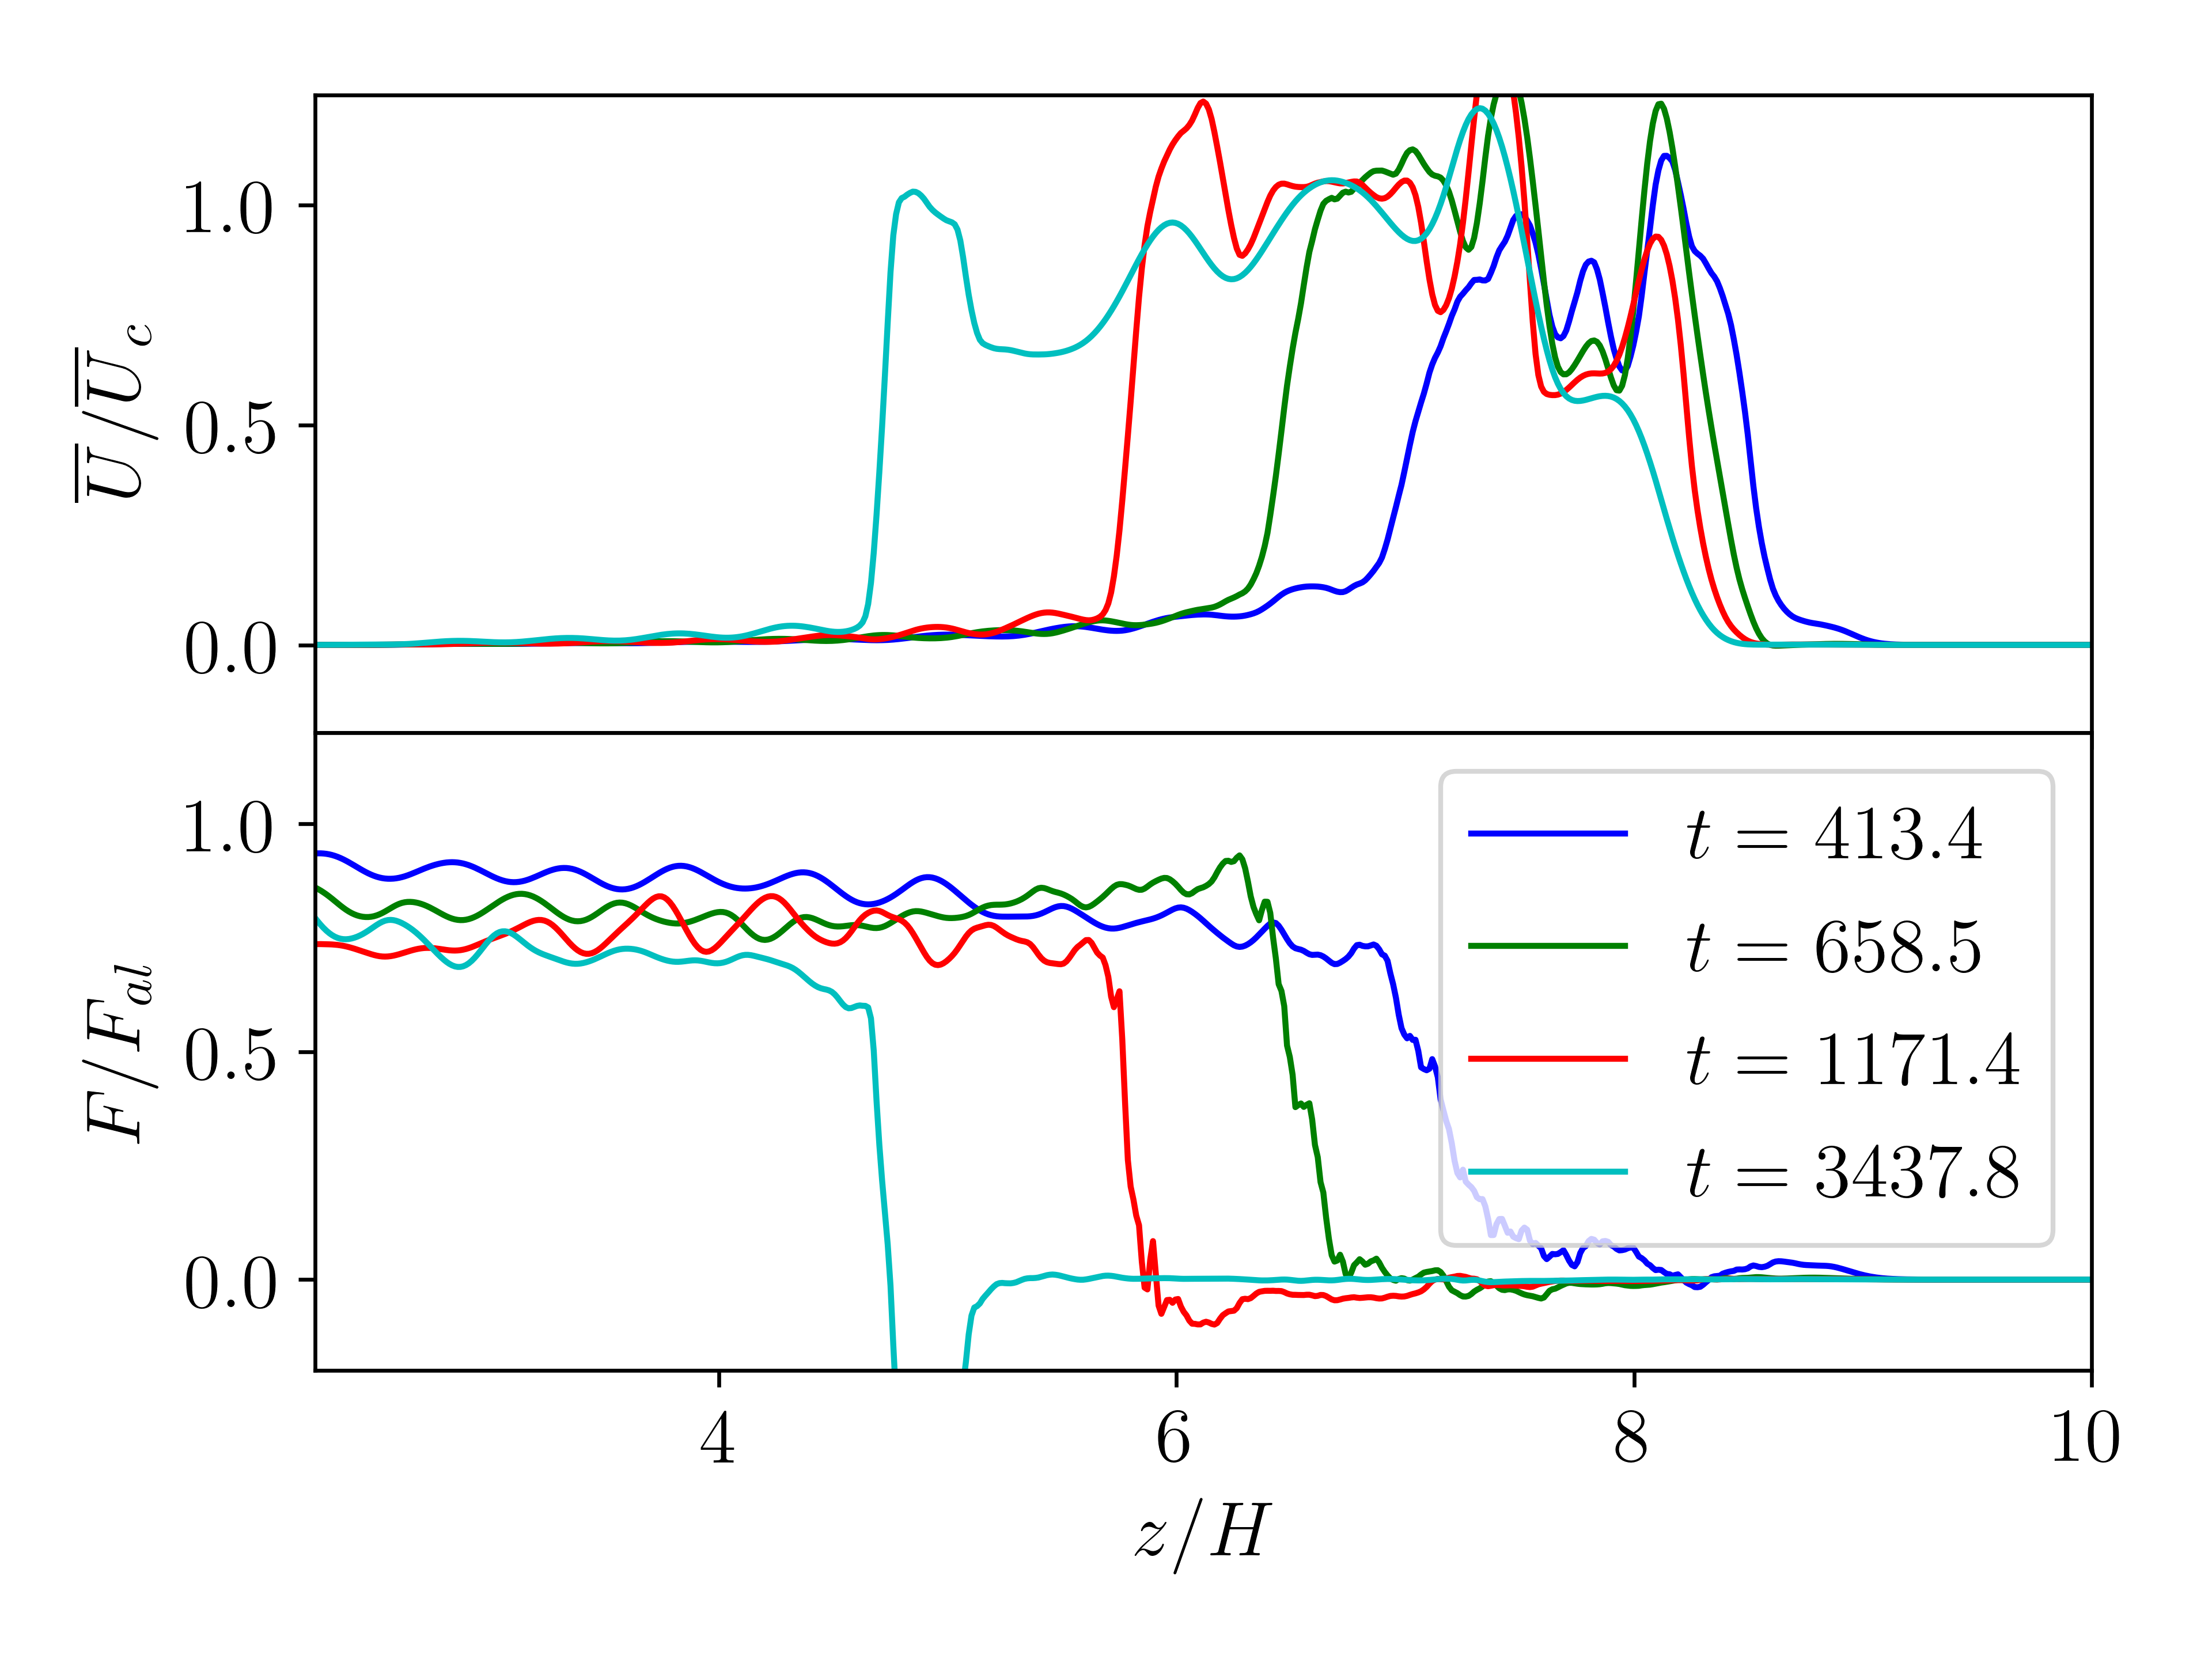
\includegraphics[width=\columnwidth]{plots/nl_fluxes.png}
    \caption{Plot of $\overline{U}(z, t)$ and $\hat{F}(z, t)$ respectively at
    various times over $z$ in our $\mathrm{Re} = 1024$ simulation.
    $\overline{U}, \hat{F}$ follow their definitions in \autoref{eq:mean_flow}
    and \autoref{eq:sbm_def}. $\overline{U}$ is given in units of
    $\overline{U}_c = \frac{\omega}{k_{x}}$ the critical horizontal flow
    velocity (see \autoref{ss:crit_layer}). The propagation of the critical
    layer towards lower $z$ and sharp deposition of $F$ at the critical layer
    are evident.}\label{fig:nl_fluxes}
\end{figure}

\subsection{Propagating Critical Layer}

For the simulation shown in \autoref{fig:nl_fluxes}, we may analyze the location
of the critical layer. As the simulations are very noisy, we measure the location
of the critical layer using an average of where flux deposition occurs
\begin{align}
    z_{c, \min} &= \argmin_z \z{z: F(z) < 0.3F_{al}'},\nonumber\\
    z_{c, \max} &= \argmax_z \z{z: F(z) > 0.3F_{al}'},\nonumber\\
    z_c &\equiv \frac{z_{c, \min} + z_{c, \max}}{2}.\label{eq:zc_def}
\end{align}
This was found to a relatively stable estimator of the critical layer location.
Other estimators were used and do not significantly change the results of the
analysis.

The evolution of $z_c$ depends on the deposited flux $\Delta F(t)$ per
\autoref{eq:zc_anal}. To estimate $\Delta F(t)$ across the critical layer $z_c$
from the data, we defined:
\begin{align}
    F_{<}(t) &= \ev{F(z)}_{z \in [z_c - \Delta z - H, z_c - \Delta z]}
        ,\label{eq:sbelow_def}\\
    F_>(t) &= \ev{\z{F(z): F(z) < 0}}_{z \in [z_c, z_c + \Delta z]},
        \label{eq:sabove_def},\\
    \Delta F(t) &\equiv F_>(t) - F_{<}(t).\label{eq:ds_def}
\end{align}
$\ev{\dots}_{z \in [z_a, z_b]}$ denotes averaging over interval $[z_a, z_b]$.
Below the critical layer, we average over an interval of length
$\frac{2\pi}{k_{z}}$ a full vertical wavelength. The offset $\Delta z$ is
necessary to make a measurement of the incident flux unaffected by the
turbulence within the critical layer itself. The height of the critical layer is
limited by $\mathrm{Ri} \lesssim 1$, which bounds its vertical extent $\sim
\frac{1}{k_{z}}$. We empirically found an offset of $\Delta z = \frac{3}{k_z}$
was necessary to be sufficiently far from strong fluctuations near the critical
layer.

Above the critical layer, waves decay over a much smaller vertical extent as
they have larger $z$ wavenumbers thanks to the shear flow Doppler shift.
Accurate measurement of these fluctuations above the critical layer is important
to measuring the transmission feature accurately, seen in
\autoref{fig:nl_fluxes} to be weak and attenuate quickly.

Finally, we may plot the measured $z_c$ against two semi-analytic predictors:
(i) integration of \autoref{eq:zc_anal} using the measured $\Delta F(t)$, and
(ii) substituting the time-averaged $\ev{\Delta F}_t$ (over the entire length of
the simulation) into \autoref{eq:zc_sol}. Since $z_c(t)$ is both stable and less
well-defined at early times (when the critical layer is thick and transient
behavior is still strong), we instead integrate backwards from the end of the
simulation, using $z_c(t_f)$ as initial condition. The resulting predictors are
depicted in \autoref{fig:nl_front}. The good agreement between the evolution of
$z_c(t)$ and its estimate via $\Delta F(t)$ and \autoref{eq:zc_anal} are
noteworthy.

Also of interest is the behavior of the time-averaged $\ev{\Delta F}_t =
0.71F_{al}'$ predictor, which serves mostly as a fiducial in the plot. The
general agreement clearly demonstrates $\Delta F < F_{al}'$ and that momentum
flux absorption is incomplete. However, its underprediction of critical layer
velocity at early times contrasts with its overprediction at later times. This
suggests that momentum flux absorption changes significantly over time, which is
in line with the observations in the subsequent \autoref{ss:reflectivity}.

\begin{figure}
    \centering
    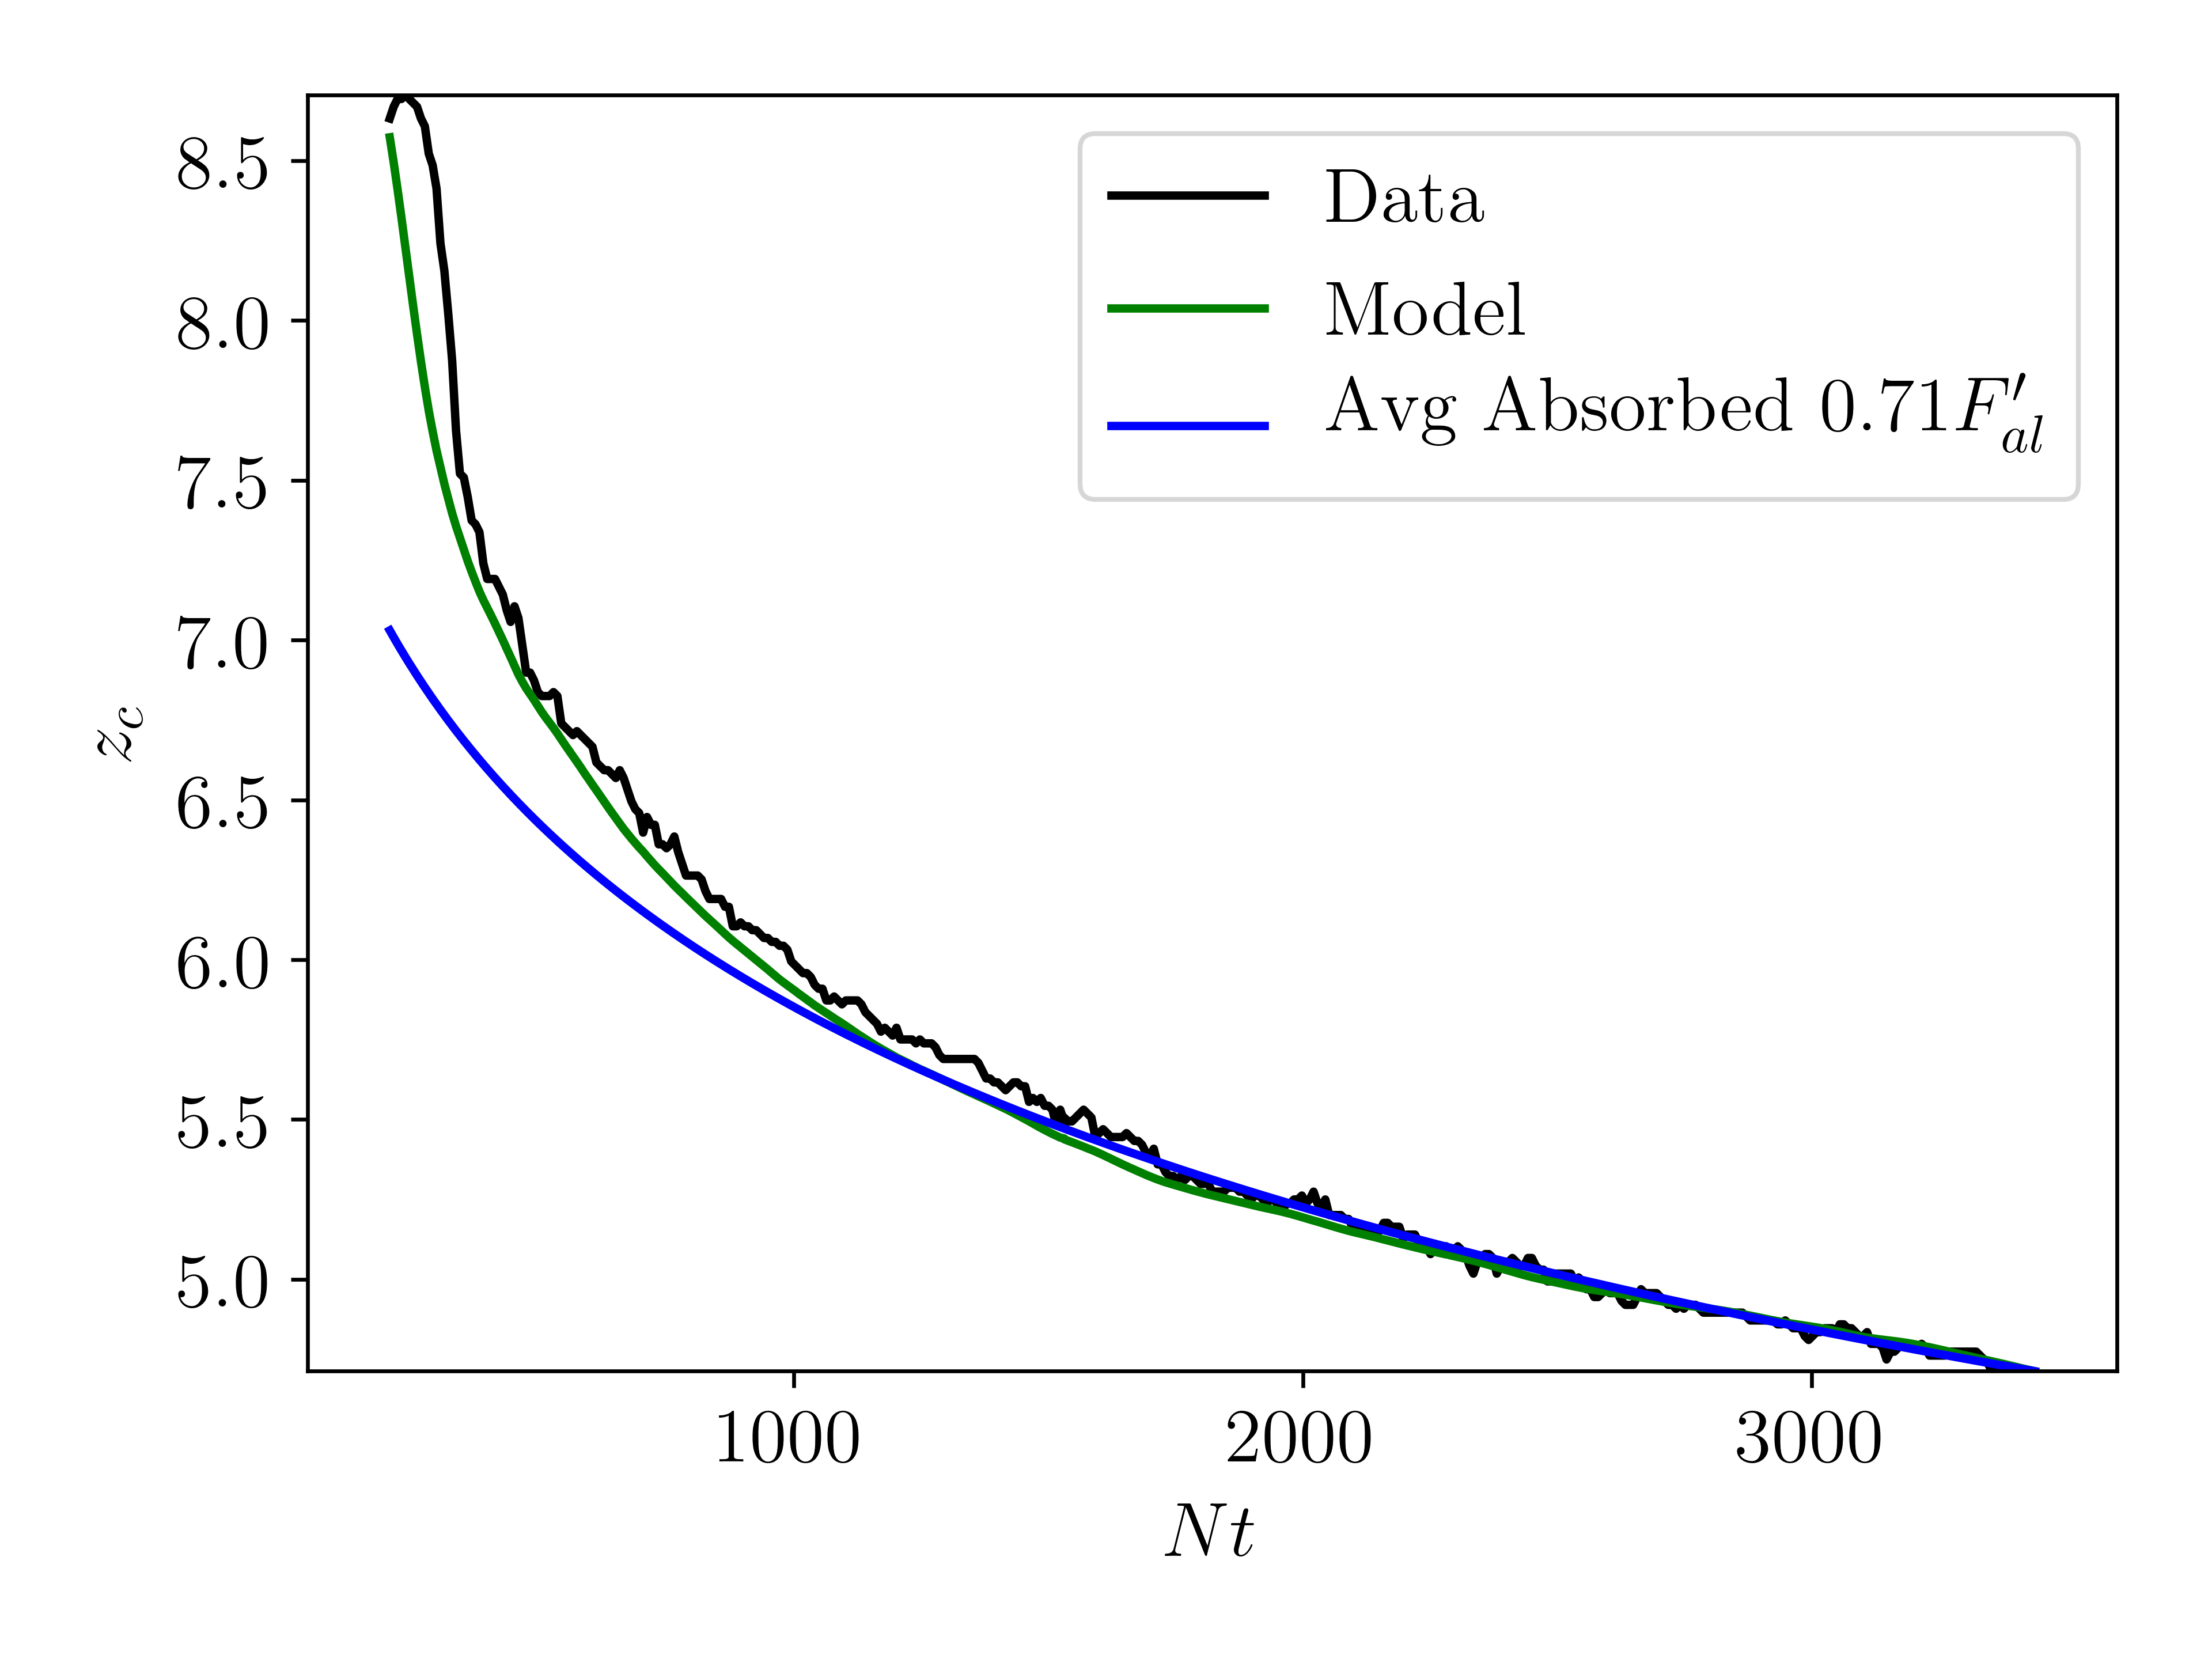
\includegraphics[width=\columnwidth]{plots/nl_front.png}
    \caption{Propagation of the critical layer over time. Shown are (black)
    $z_c(t)$ from simulation data, (green) predictor of $z_c(t)$ using direct
    integration of \autoref{eq:zc_anal} for $\Delta F(t)$ measured from
    simulation data (described in \autoref{eq:ds_def}) and (blue) direct
    substitution of time-averaged $\ev{\Delta F(t)}_t$ into
    \autoref{eq:zc_sol}. Predictors use the end of the simulation as initial
    conditions and integrate backwards, as $z_c$ is less well-defined at early
    times. The agreement of the directly-integrated predictor with the data
    shows \autoref{eq:zc_anal} is a good description of the evolution of $z_c$.
    The the poorer but qualitatively correct agreement of the time-averaged
    predictor with the data shows both that $\Delta F(t) \neq F_{al}'$ and that
    $\Delta F(t)$ likely has some very real variation with
    time.}\label{fig:nl_front}
\end{figure}

\subsection{Kelvin-Helmholtz Instability and Critical Layer Width}\label{ss:khi}

The observation of reflected/transmitted waves is in accordange with previous
studies as discussed in \autoref{ss:wave_breaking}. Studies have shown that a
local Richardson number $\mathrm{Ri} \sim 1/4$ corresponds to the onset of
reflectivity. This $\mathrm{Ri}$ also corresponds to the onset of the
Kelvin-Helmholtz instability (KHI). Indeed, in our simulations, visual
inspection suggests the KHI is present in the critical layer (see
\autoref{fig:snapshots}). It is natural to suspect then that the shear flow
cannot steepen any further than KHI onset. To verify this, we decided to compute
a local $\mathrm{Ri}$ for the shear flow around the critical layer.

Since fluid instabilities are local, $\mathrm{Ri}$ must be measured in the
immediate vicinity of a fluid parcel. Thus, we first assign an $\mathrm{Ri}$ for
every $x$ in the critical layer, then take the median as $\mathrm{Ri}$ for the
entire layer. To avoid noisiness, the local $\mathrm{Ri}$ is computed using the
vertical distance over which the local $u_x$ increases from $0.3 \times$ its
critical value to its critical value. The value $0.3$ effectively excludes the
self-acceleration induced by the IGW\@. This can be written
\begin{align}
    z_{CL, \min}(x, t) &= \argmin_\zeta
        \z{z: u_x(x, \zeta, t) > 0.3\overline{U}_c},\nonumber\\
    z_{CL, \max}(x, t) &= \argmax
        \zeta \z{z: u_x(x, \zeta, t) < \overline{U}_c},\nonumber\\
    \mathrm{Ri}(t) &\equiv
        \med_x\p{\frac{N^2 \p{z_{CL, \max} - z_{CL, \min}}^2}{(0.7
            \overline{U}_c)^2}}.\label{ss:ri_med_def}
\end{align}
To understand the variation in $\mathrm{Ri}$ over $x$, we can also plot using
the minimum over $x$ (the maximum is significantly noisier). Both of these are
shown in \autoref{fig:nl_f_ri}. The quick evolution of $\mathrm{Ri}$ to its
saturated value is reflective of the fact that IGW are \emph{anti-diffusive}.
This property is a simple consequence of the IGW dispersion relation
\autoref{eq:disp_rel}, which is approximately $\omega k_z \approx Nk_x$ such
that as an IGW propagates into a shear flow, $\omega$ decreases and $k_z$
increases, enhancing dissipation and further driving mean flow acceleration.
\begin{figure}
    \centering
    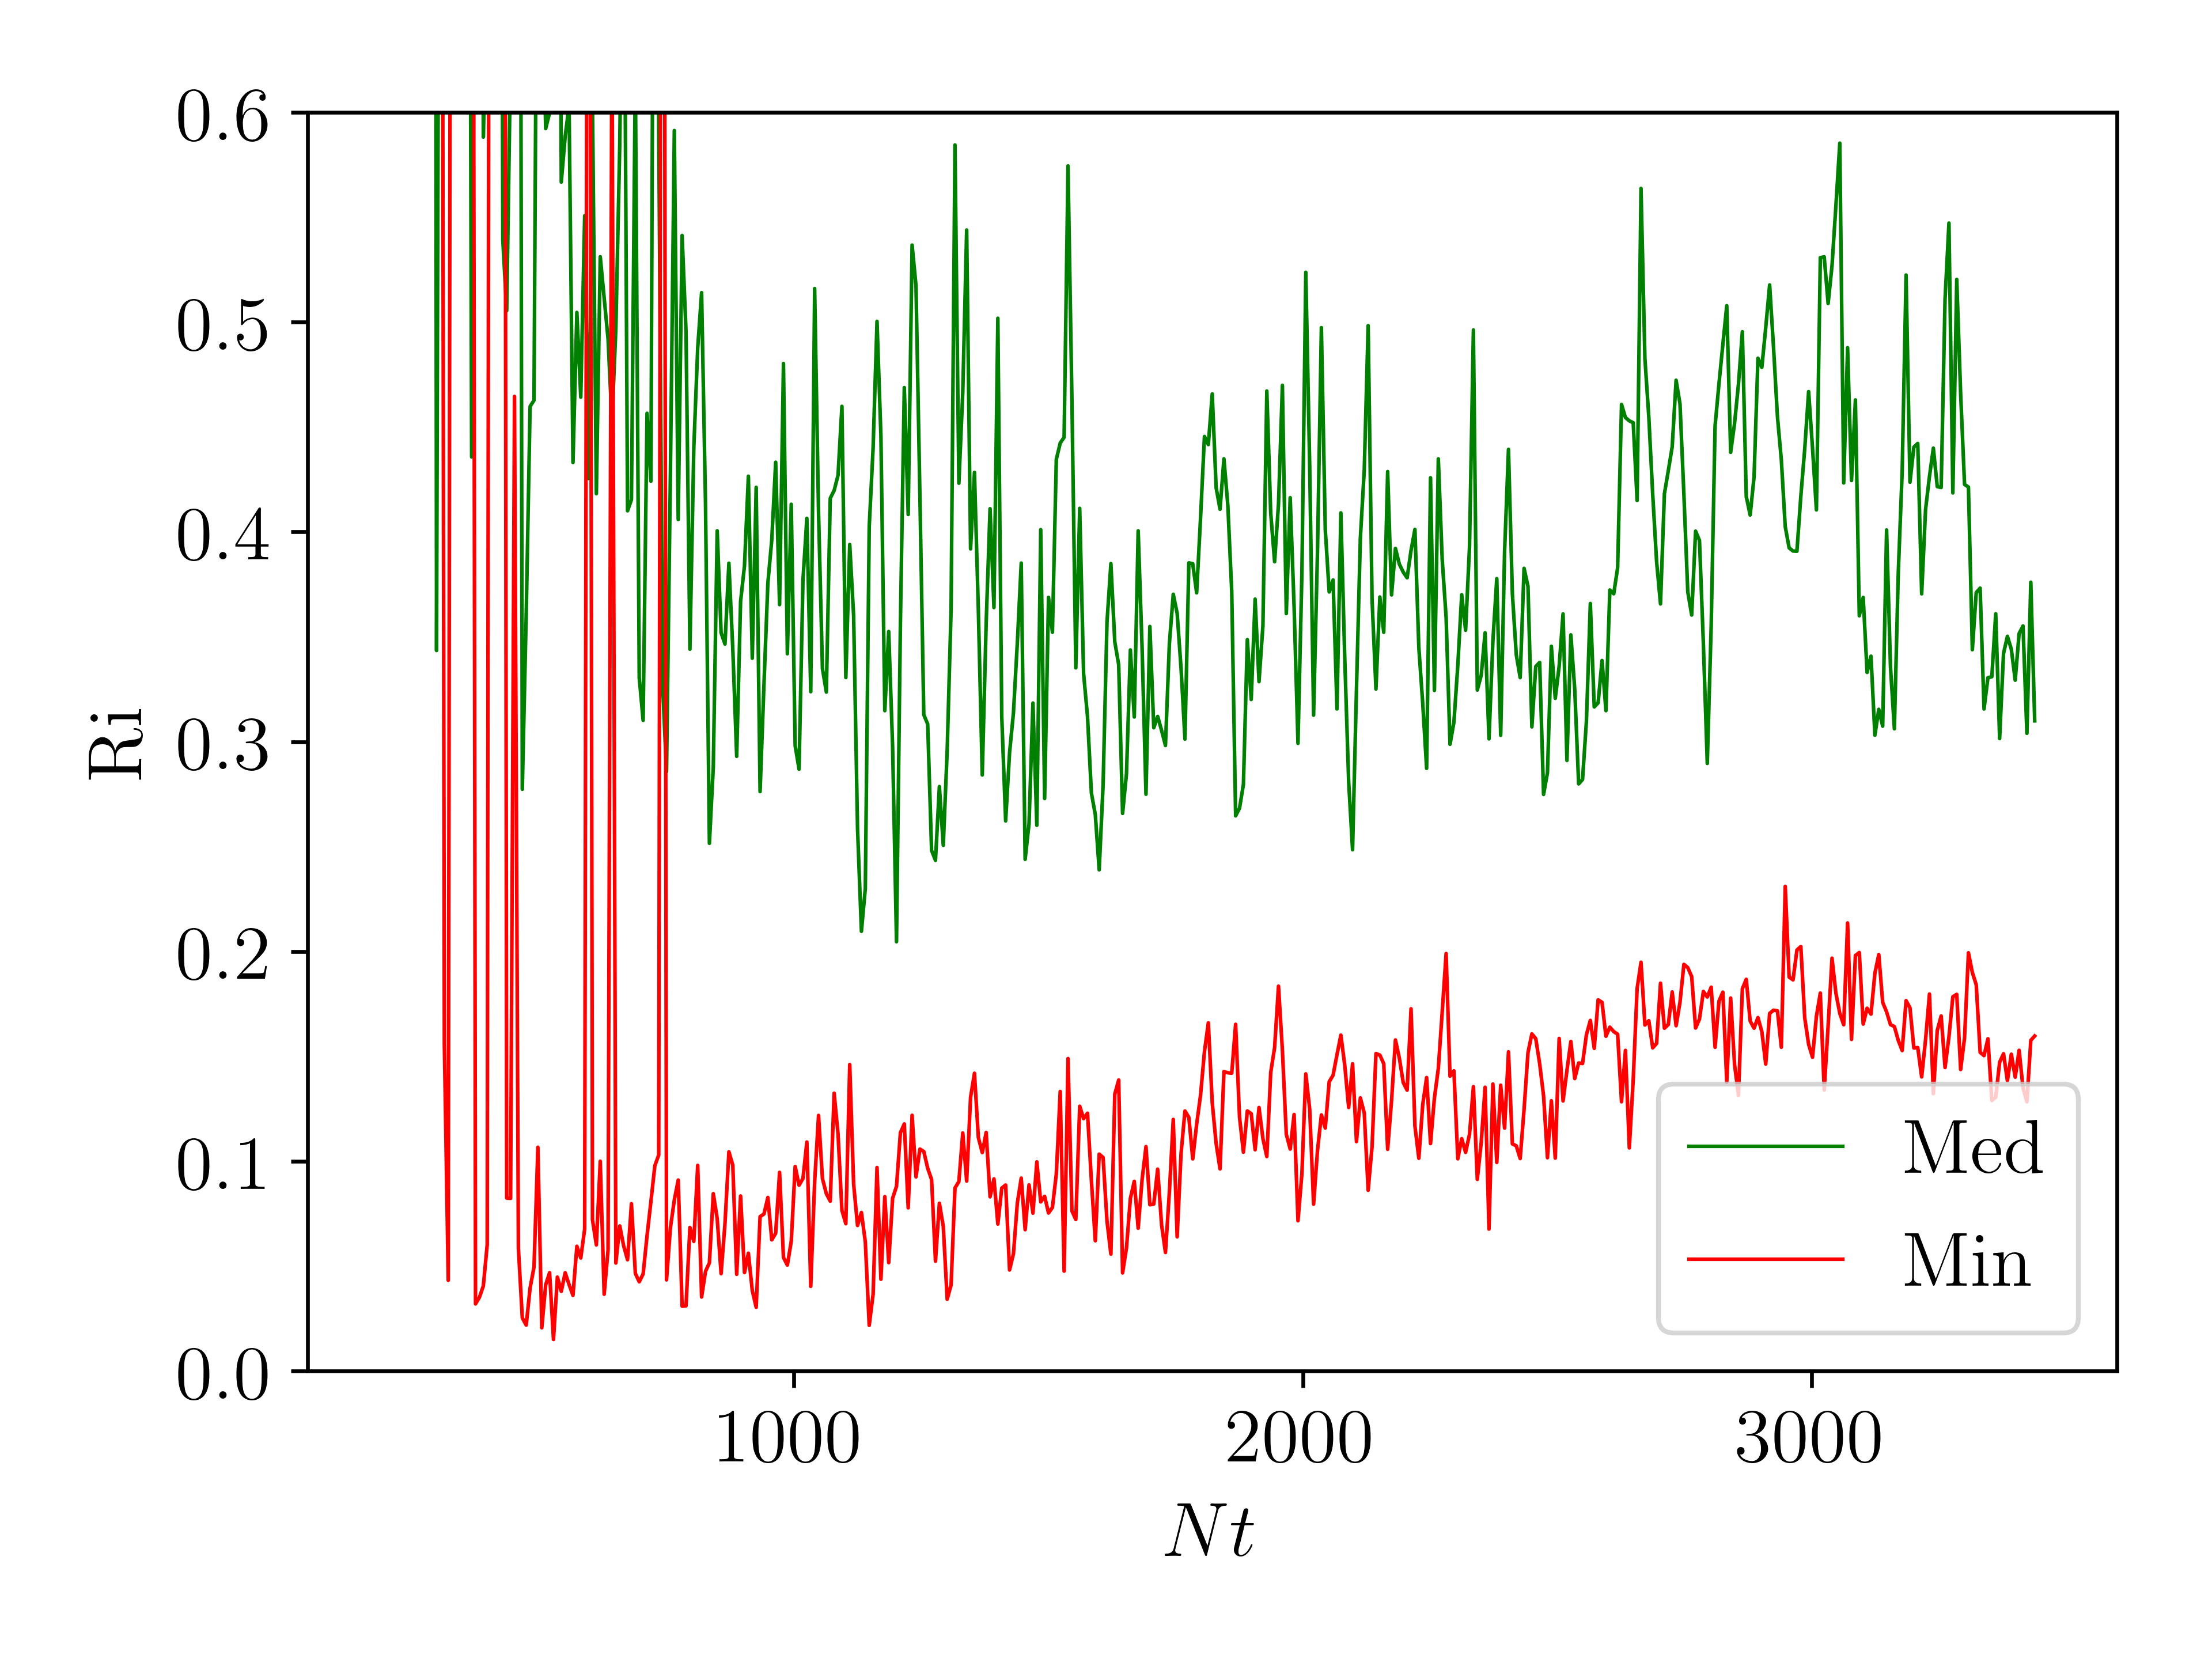
\includegraphics[width=\columnwidth]{plots/nl_f_ri.png}
    \caption{Local Richardson number of the flow at the critical layer over time
    as defined in \autoref{ss:ri_med_def}. Dotted red lines demarcate the
    minimum and median of $\mathrm{Ri}$ over $x$. These numbers effectively
    measure the mean and spread in width of the critical layer over $x$. Note
    that $\mathrm{Ri} \sim \frac{1}{4}$ corresponds to the KHI, so this plot
    suggests the shear at the critical layer does not steepen past the KHI
    onset.}\label{fig:nl_f_ri}
\end{figure}

\subsection{Non-absorption at Critical Layer}\label{ss:reflectivity}

We identify two manifestations of non-absorptive behavior: (i), the presence of
a reflected wave with wave vector $\bm{k} = k_{x}\uv{x} - k_{z}\uv{z}$, and (ii)
the amount of horizontal momentum flux $F$ reflected/transmitted by the critical
layer. The reflected wave amplitude and reflected flux need not agree exactly if
some reflected flux is in higher-order modes, which is indeed the case in our
simulations. Both are of physical interest, however: the reflected wave
amplitude may be of physical interest in setting up standing modes in a
realistic star, while the flux transfer properties is important for accurately
tracking angular momentum transfer during synchronization.

To measure the reflected wave amplitude, we use almost the same definition
\autoref{eq:ahat_def} except using $k_{z} \to -k_{z}$; call this estimated
$\hat{A}_r(t)$ the amplitude of the downwards-propagating reflected wave. To
compute $\hat{A}_r(t)$, we furthermore permit an arbitrary phase offset
$\phi_r(t)$ at each time $t$, since the phase of the reflected wave is unknown,
unlike that of the incident wave. $\phi_r(t)$ in our simulations
behaves in agreement with reflection off a moving boundary at $z_c$,
well approximated by $\abs{\pd{\phi_r}{t}} \approx 2\abs{\pd{(k_{z}z_c)}{t}}$.

Since reflectivity depends sensitively on accurate measurements of $\hat{A}_i,
\hat{A}_r$, we remark \autoref{eq:ahat_def} ensures orthogonality between
$k_{x}\uv{x} \pm k_{z}\uv{z}$ modes. The integral for $\hat{A}_r$ is also
performed over $z \in [z_0 + 3\sigma, z_0 + 3\sigma + H]$. Since
$\hat{A}_i(t), \hat{A}_r(t)$ vary somewhat strongly over time, we perform time
averaging over interval approximately $8\pi/\omega$, denoted by angle brackets.
We can then define the amplitude reflectivity
\begin{equation}
    \mathcal{R}_A(t) \equiv \frac{\ev{\hat{A}_r}(t)}{\ev{\hat{A}_i}(t)}
        .\label{eq:Ra_def}
\end{equation}
% 7/N per timestep, 13 timestep smoothing kernel, 24/N period

To measure the reflected horizontal momentum flux, we recall from our linear
simulations described in \autoref{ss:lin_ns} that we are able to accurately
predict the incident flux from the incident wave amplitude. Thus, we write for
incident flux
\begin{equation}
    F_i(t) \equiv \ev{\rho u_{x} u_{z}}_x\hat{A}_i^2(t).
\end{equation}
But then, since we already have $\Delta F(t), F_>(t)$ jump and transmitted flux
across the critical layer at time $t$ respectively, we can immediately write
down the reflected flux
\begin{equation}
    F_r(t) = F_i(t) + \Delta F(t) - F_>(t).
\end{equation}
Note that $F_>(t)$ is just the transmitted flux across the critical layer, since
there is no other flux above the critical layer. We then define flux
reflectivity and transmissivity coefficients
\begin{align}
    \mathcal{R}_F(t) &\equiv -\frac{\ev{F_r}(t)}{\ev{F_i}(t)},&
    \mathcal{T}_F(t) &\equiv -\frac{\ev{F_>}(t)}{\ev{F_i}(t)}.
        \label{eq:srefl_def}
\end{align}

The measurements of $\hat{A}_i, \hat{A}_r, F_i, \Delta F, F_r, F_>$ are given in
\autoref{fig:nl_f_amps}. The oscillations in $\hat{A}_i, F_i, A_d, F_r$ are
significant but the mean values seem to have temporally converged.

\begin{figure}
    \centering
    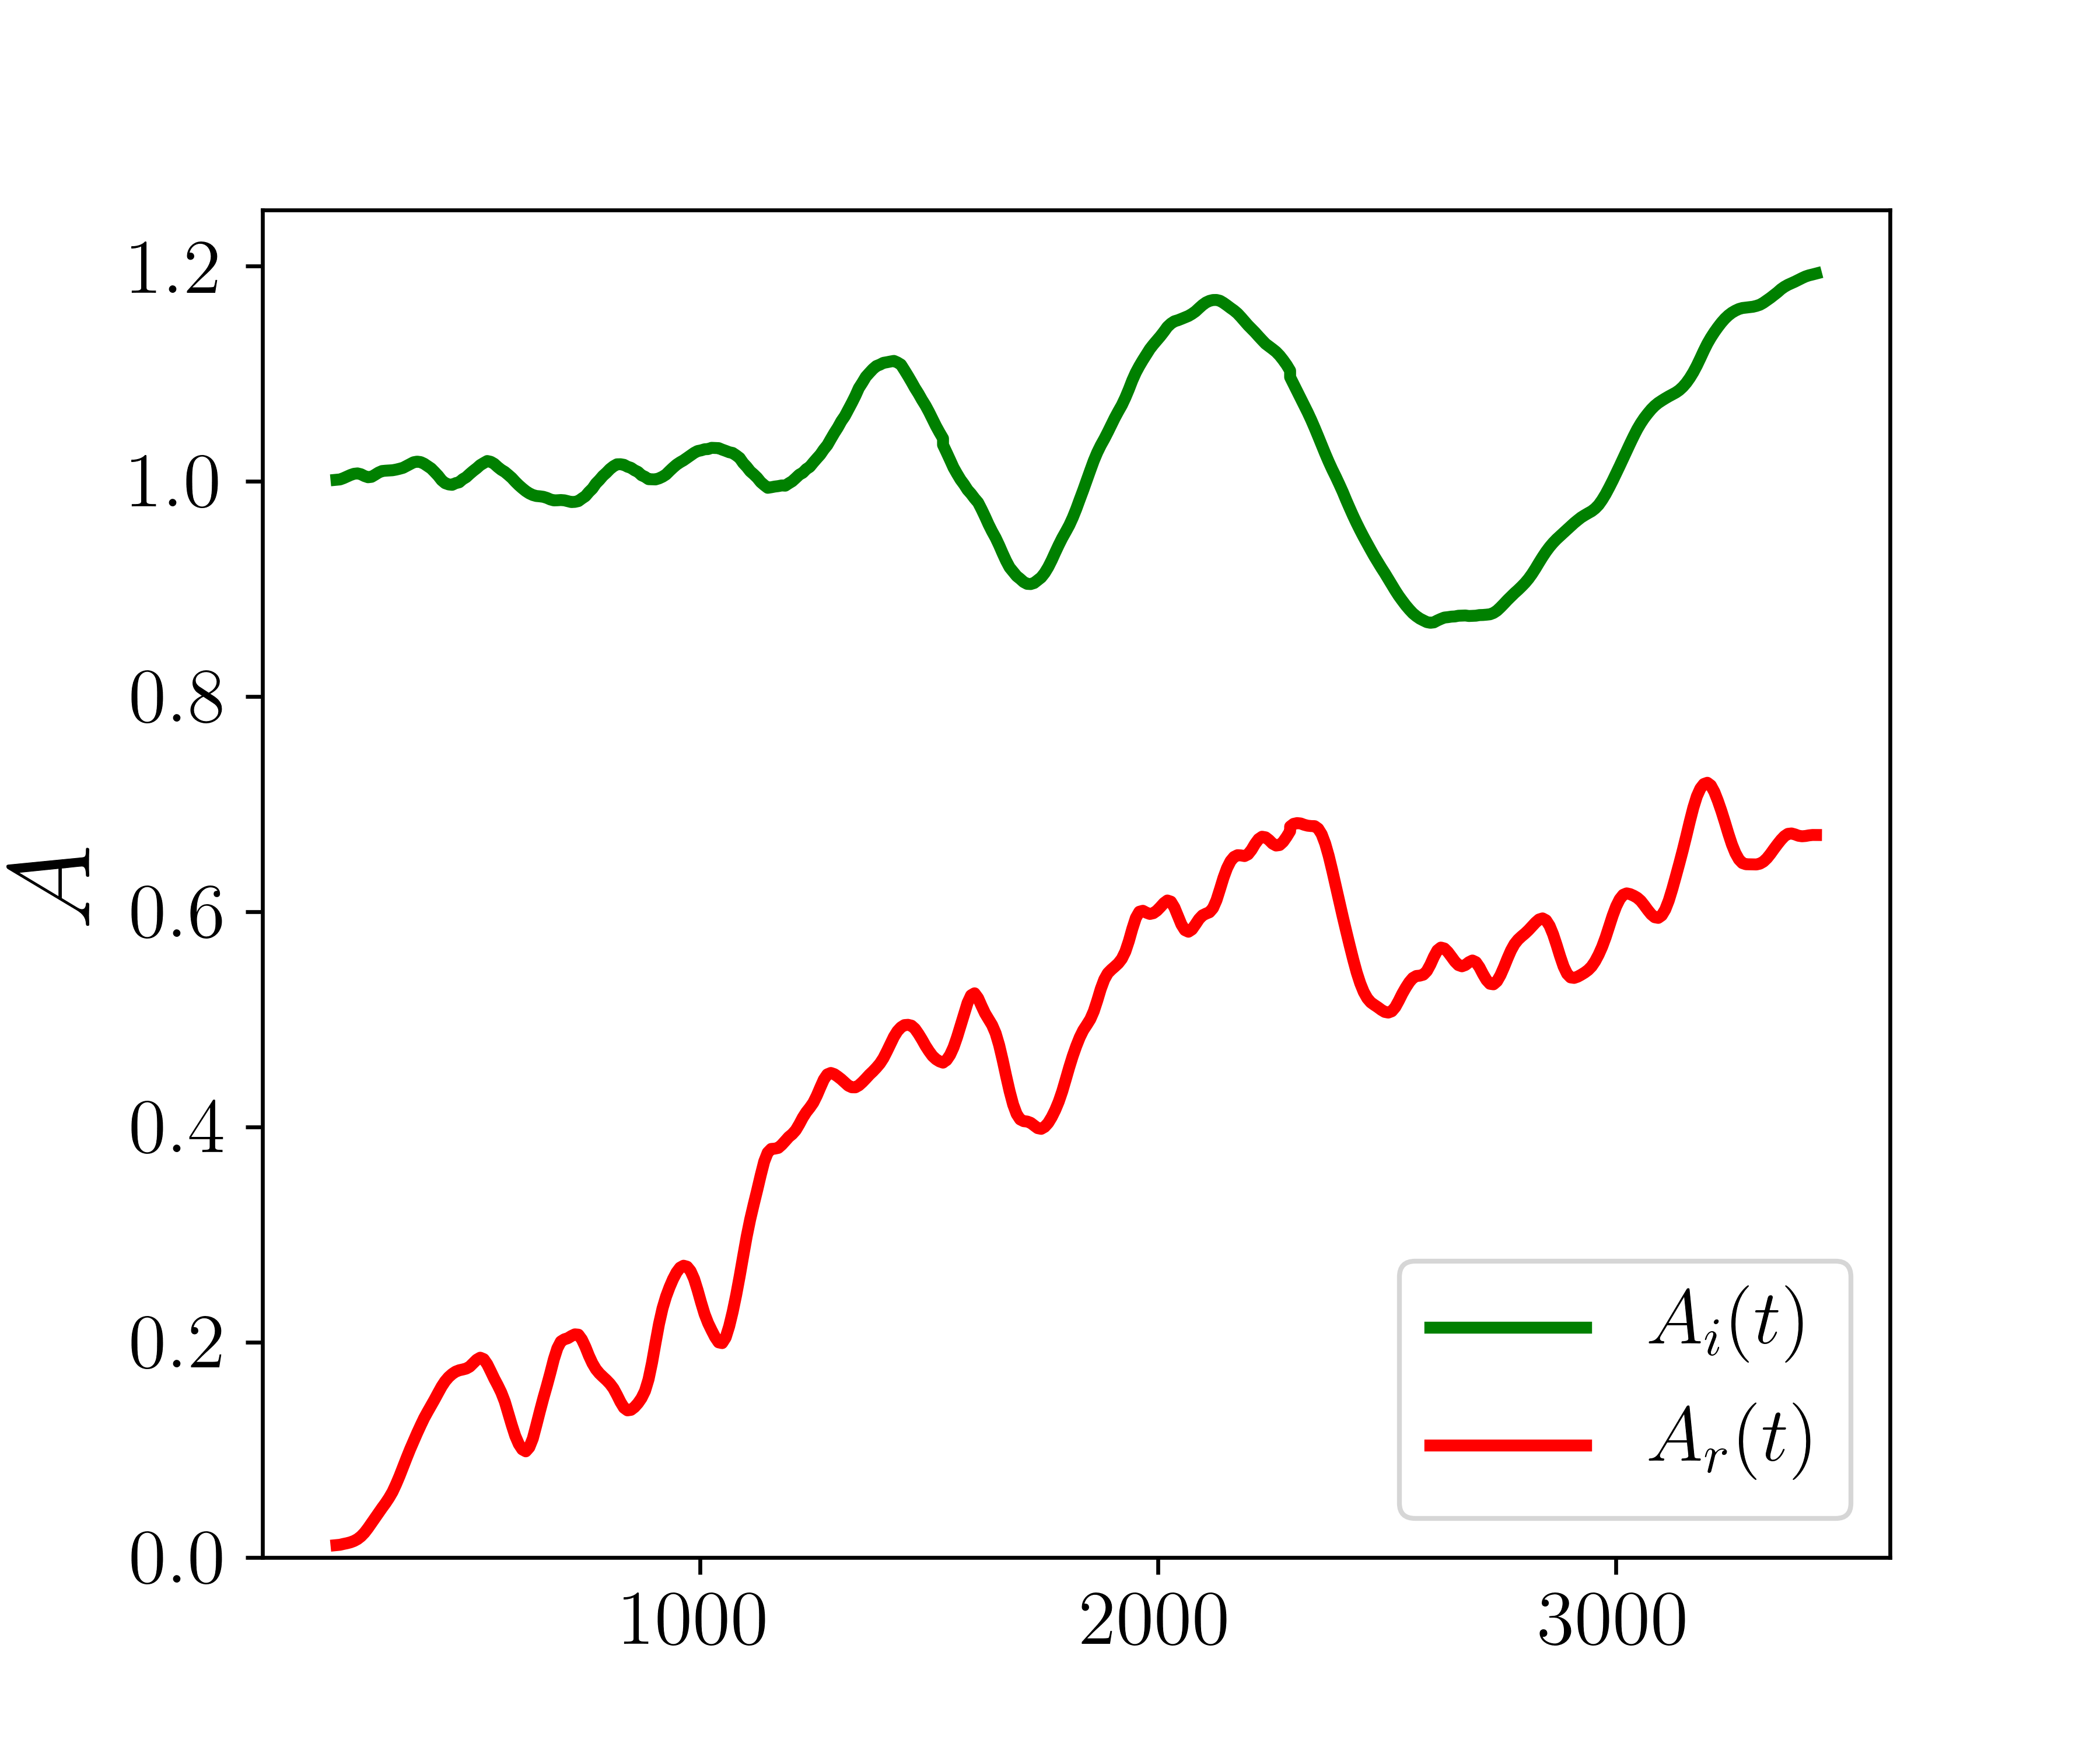
\includegraphics[width=\columnwidth]{plots/nl_f_amps.png}
    \caption{The top panel measures the incident wave amplitude $\hat{A}_i(t)$
    (green) and the downwards propagating wave amplitude $\hat{A}_r(t)$ (red)
    just above the forcing zone, normalized to the analytical estimate
    \autoref{eq:uz_lin}. $A_d \neq 0$ due to reflection off the critical layer.
    The bottom panel shows the behavior of three horizontal momentum fluxes over
    time, in units of the analytical estimate \autoref{eq:S_lin}: (blue) flux
    incident on the critical layer, (red) flux absorbed by the critical layer,
    and (black) flux transmitted through the critical
    layer.}\label{fig:nl_f_amps}
\end{figure}

Using these measured quantities, we may make plots of $\mathcal{R}_A^2,
\mathcal{R}_F, \mathcal{T}_F$, which are provided in \autoref{fig:nl_f_refl}. A
comparison between $\mathcal{R}_A^2$ and $\mathcal{R}_F$ is appropriate as $F
\propto A^2$. Visual inspection suggests the three quantities have reached
their asymptotic values after $t \gtrsim 1750/N$. An observation may be made
that in general $\mathcal{R}_F \geq \mathcal{R}_A^2$; this conforms to the
expectation that reflected flux consists of the simple reflected mode and higher
order modes as well.

\begin{figure}
    \centering
    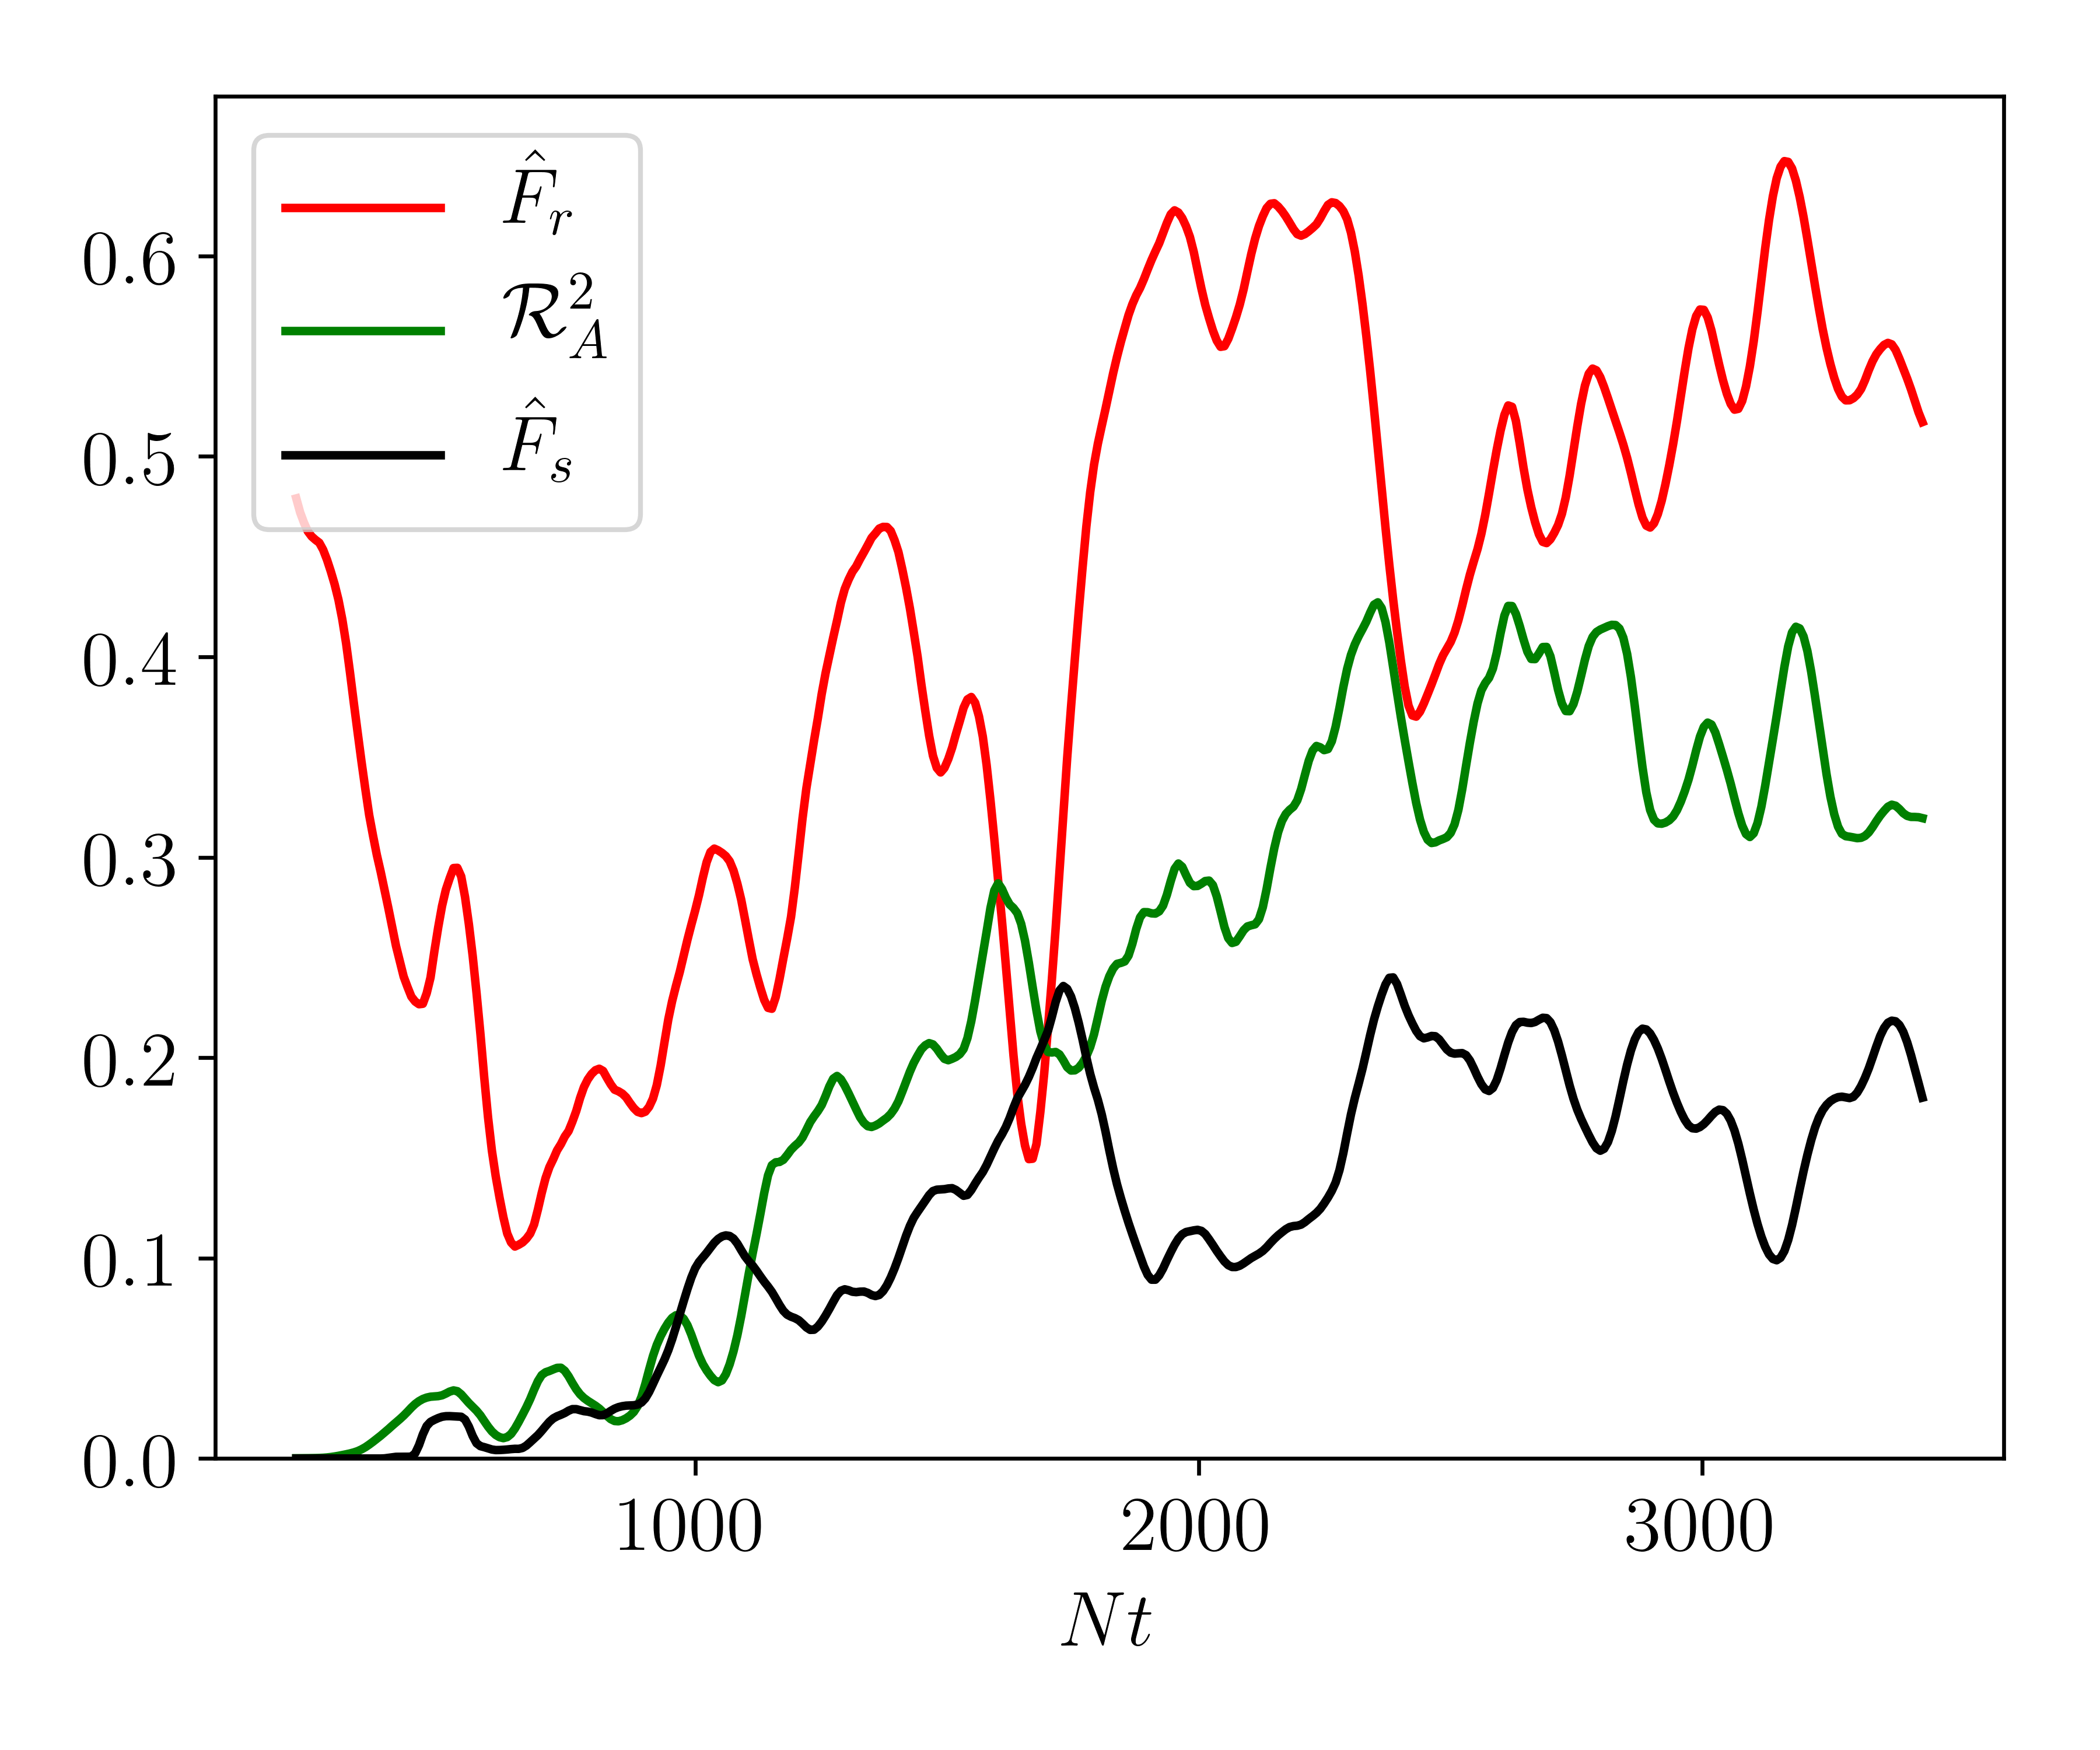
\includegraphics[width=\columnwidth]{plots/nl_f_refl.png}
    \caption{Reflectivity and transmittivity coefficients for flux and
    amplitude-squared as described by \autoref{eq:Ra_def} and
    \autoref{eq:srefl_def} respectively. The coefficients seem to become
    comparatively stable past about $t = 1750/N$, indicating that an asymptotic
    value may have been reached.}\label{fig:nl_f_refl}
\end{figure}

\subsection{Convergence}\label{ss:convergence}

As the primary test of convergence in our previous sections, we consider the
convergence of the physically significant parameters of our model. In
particular, the convergence of $\mathrm{Ri}$, shown in \autoref{fig:nl_f_ri},
and of the reflection/transmission coefficient asymptotic values, shown in
\autoref{fig:nl_f_refl}, are of greatest significance.

To estimate convergence, we compute the median value of each of $\mathrm{Ri},
\mathcal{R}_A^2, \mathcal{R}_F, \mathcal{T}_F$ over the last $1/4$ of simulation
times from each simulation, where all simulations had converged to what appeared
to be asymptotic values. Error bars are estimated with the $16$ and $84$
percentiles. We illustrate the convergence of these averages across simulations
in \autoref{fig:agg}.
\begin{figure}
    \centering
    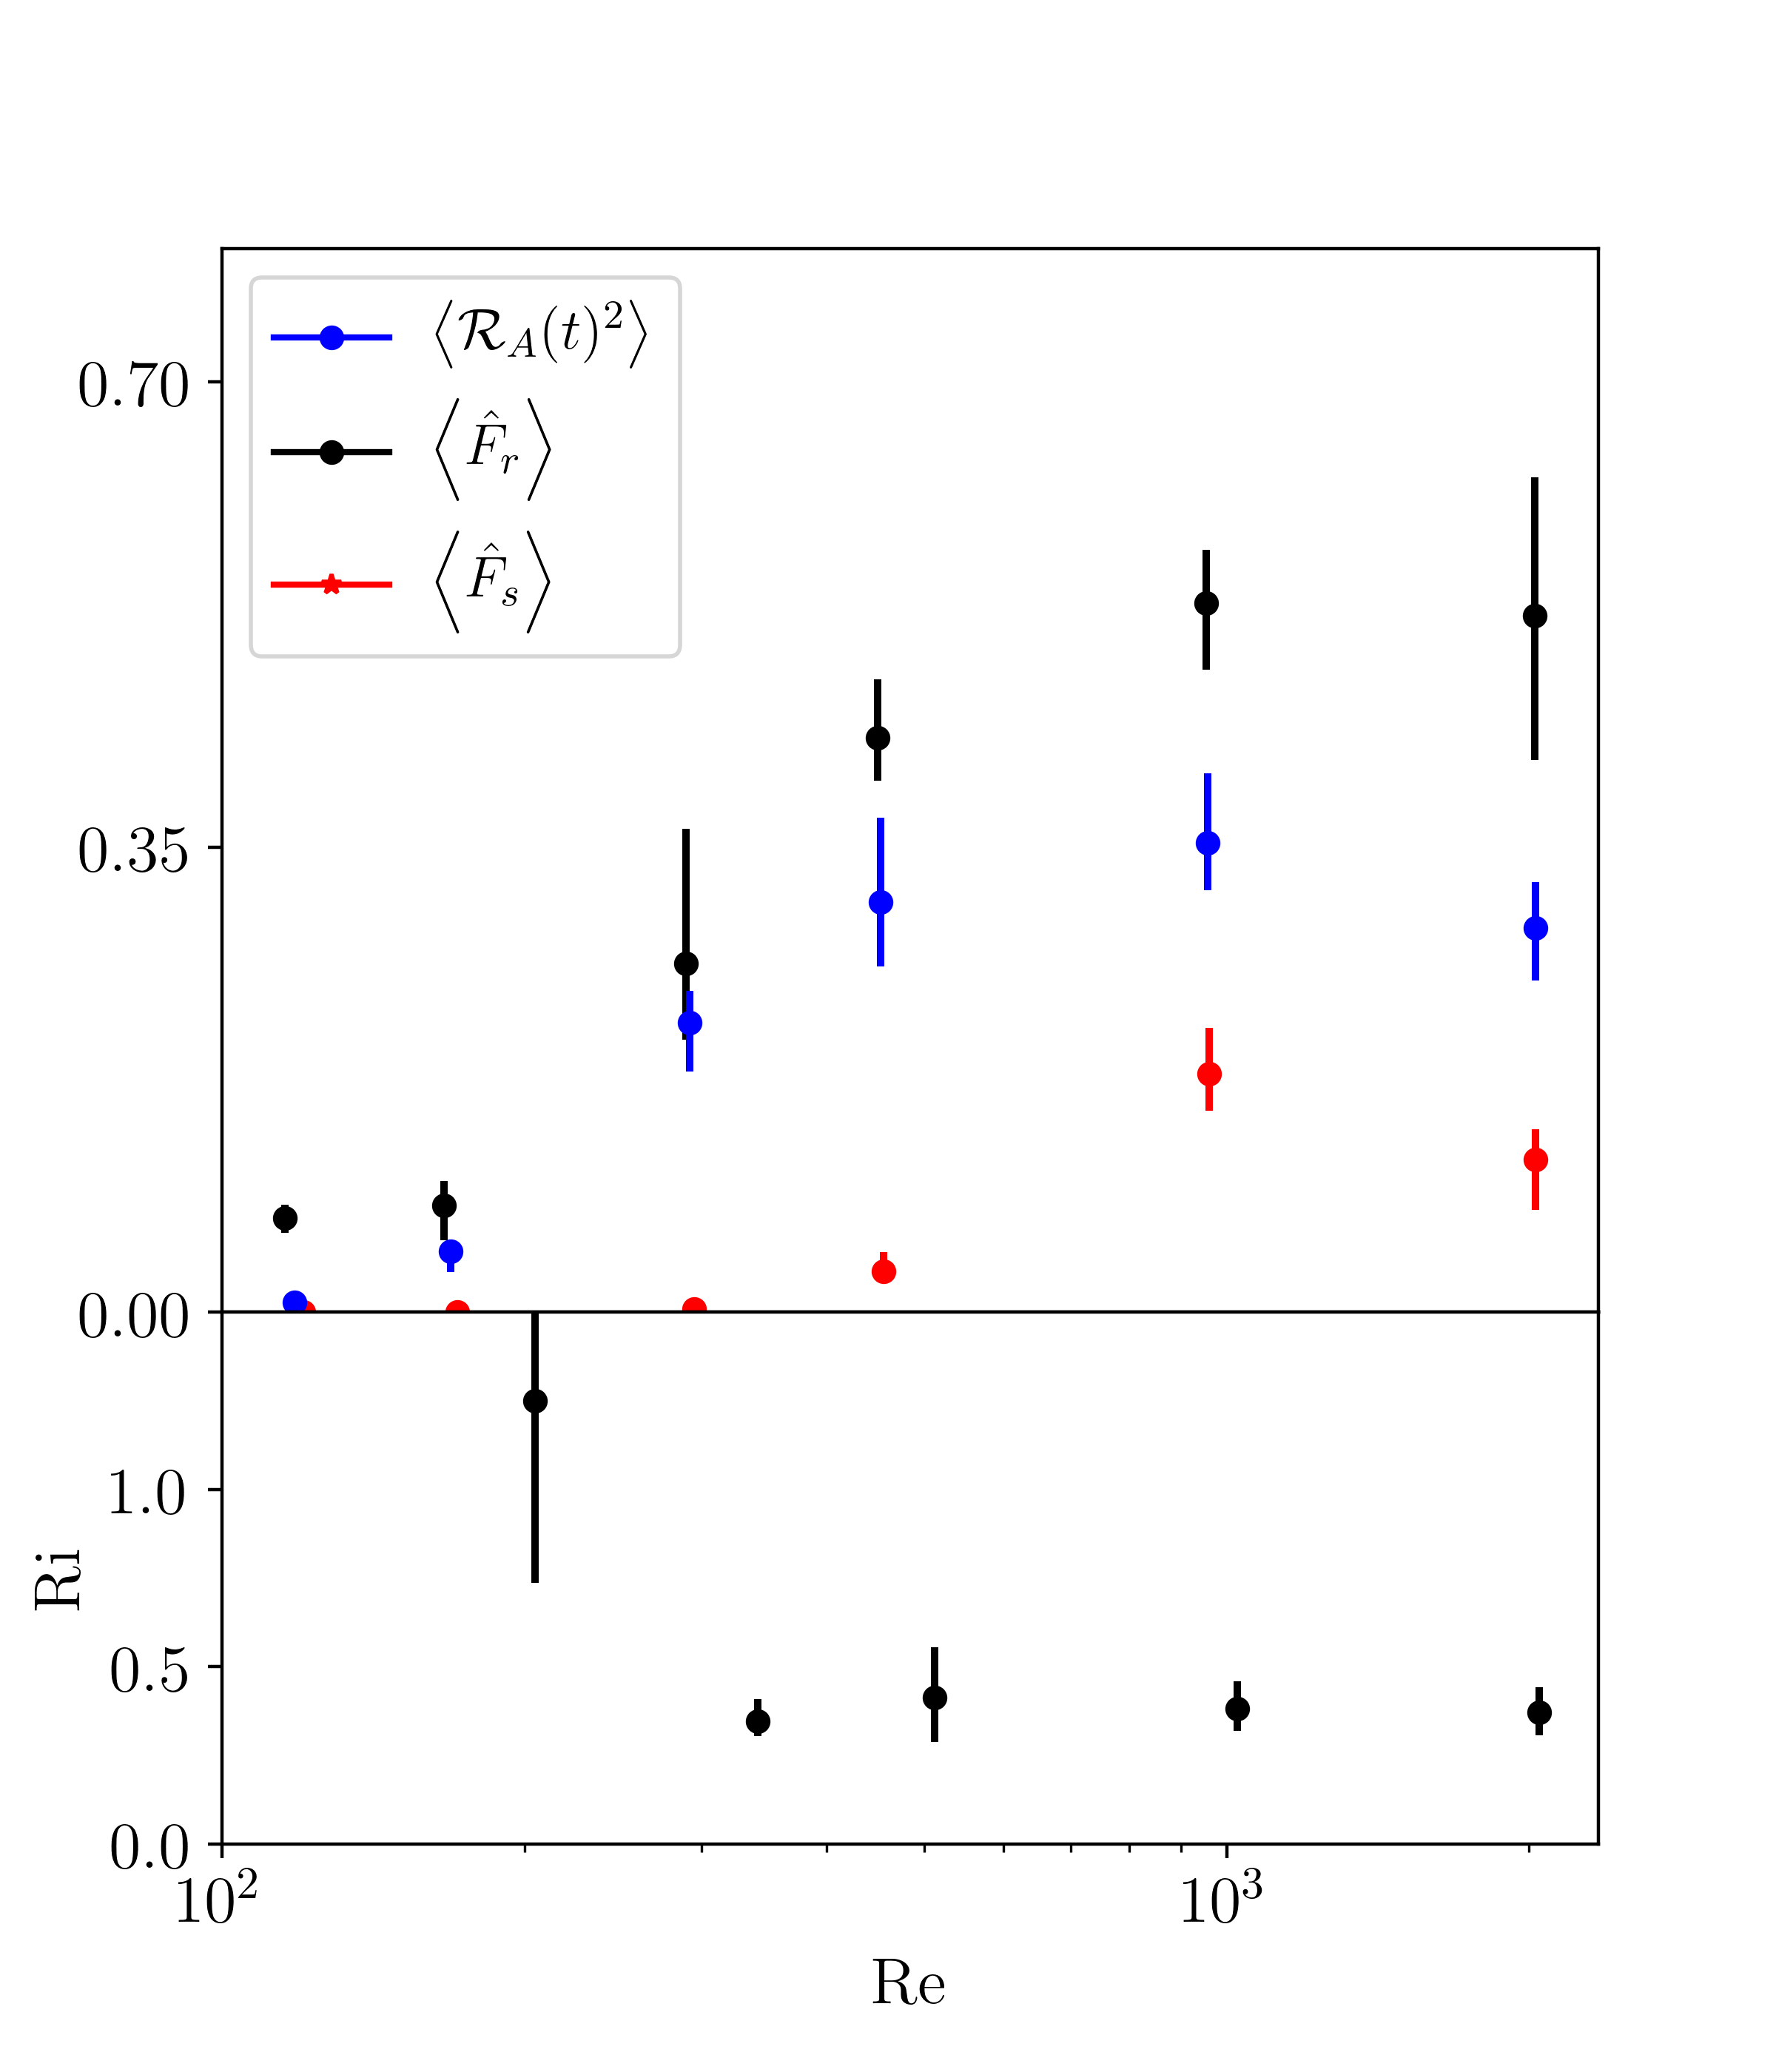
\includegraphics[width=\columnwidth]{plots/agg.png}
    \caption{Convergence of median reflection/transmission coefficients and
    $\mathrm{Ri}$ (critical layer width) across runs with varying viscosity,
    parameterized with $\mathrm{Re}$ (\autoref{eq:re_def}). Error bars depict
    $16$ and $84$ percentile values. Small horizontal displacements are made for
    data points at identical $\mathrm{Re}$ for readability. Note that
    simulations with larger $\mathrm{Re}$ correspond to smaller viscosity and
    are more physically realistic, and our values seem to converge towards large
    $\mathrm{Re}$. At the smallest $\mathrm{Re}$ value, $\mathrm{Ri} \approx 50$
    is too large to fit on the plot.}\label{fig:agg}
\end{figure}

It is apparent that the Richardson number rapidly converges to $\mathrm{Ri}
\approx 0.4$ but the reflection/transmission coefficients converge more slowly.
This is in disagreement with \autoref{eq:crit_coeffs} calculated via the linear
analytical theory. This tension is natural: fluid motion within the critical
layer is turbulent, so transmission/reflection at the critical layer cannot be
captured by any linear theory.

\section{Discussion}\label{s:discussion}

In the previous section, we have argued for a continous train of breaking IGWs
spontaneously forming a critical layer and strong shear flow. We have
parameterized the width of the critical layer as well as horizontal momentum
transport near the critical layer. In the subsequent sections, we will discuss
the validity of these results and their application to astrophysical systems.

\subsection{Physical Sources of Dissipation in WDs}\label{ss:disp}

The most significant linear damping in WD g-modes comes from radiative damping
\citep{fullerI}. In \citep{wu} and \citep{fullerI}, the radiative damping rate
is given in terms of $\omega_i = \gamma \omega_r$, where $\omega_r$ is the
frequency of the g-mode. Typical values for $\gamma$ range from $10^{-4}$ to
$10^{-11}$ depending on $n$ of the g-mode.

We will assume this prescription directly transfers to propagating IGW, which
results in general agreement with \citep{bukart}'s estimate of radiative damping
rates. Then, making coarse identification $\omega_i \sim \nu k^2 \approx \nu
k_z^2$, we find that $\mathrm{Re} \sim \frac{1}{\gamma}$. Even at $\gamma =
10^{-4}$ however, the corresponding $\mathrm{Re}$ is far too weak to suppress
reflection/transmission at the critical layer (e.g.\ \autoref{fig:agg}).

Another source of dissipation considered in \citep{bukart} is turbulent
conbmtive damping. They find this damping rate to never exceed that of
radiative damping, and so it is also too weak to suppress critical layer
formation in our problem.

Finally, we consider the impact of magnetic winding. In \citep{bukart}, magnetic
winding is used to enforce solid body rotation on the grounds that $t_A \gg
t_{gw}$, where
\begin{equation}
    t_A = \int\limits_0^R \frac{\sqrt{4\pi \rho}}{B_0}\;\mathrm{d}r
        \sim 10^2\;\mathrm{yr}\p{\frac{10^3\;\mathrm{G}}{B}}.
\end{equation}
the Alfv\'en wave crossing time (evaluated for a CO WD in \citealt{fullerIV})
measures the magnetic coupling time and $t_{gw}$ measures the gravitational wave
inspiral timescale. Before solid body rotation is attained, another relevant
timescale is the synchronization timescale $t_s$. For a tidal torque $\tau$ and
tidal forcing frequency $\sigma = m\p{\Omega - \Omega_{spin}}$, we note that
angular momentum transfer is $\pd{M_{sync}}{t} \sigma R^2 = \tau$, where
$M_{sync}$ denotes the mass of the WD that has synchronized. Thus, the
synchronization timescale is
\begin{align}
    t_{sync} &\sim \frac{M_{sync}\sigma R^2}{\tau},\nonumber\\
        &\sim 2 \times 10^5\;\mathrm{yr}
            \p{\frac{M}{M_{\odot}}}
            \p{\frac{\sigma}{2\pi / (1\;\mathrm{hr})}}
            \p{\frac{R}{R_{\oplus}}}^2
            \p{\frac{10^{-14} GM_{\odot}^2/R_{\oplus}}{\tau}}.
\end{align}
A representative $\tau$ has been taken from \citep{bukart}. However, since only
the outer $\sim 10^{-4}M_{\odot}$ need be heated for the thermodynamically
interesting effects studied in \citep{fullerIV} and \citep{tidal_novae}, it
seems that magnetic winding cannot absolutely rule out energetic outbursts such
as tidal novae resulting from strong shear flows.

\subsection{Applicability to Other Astrophysical Systems}

[TODO flesh out]

\begin{itemize}
    \item $k_x, k_z$: In astrophysical systems, $k_{\perp} \ll k_r$. While we do
        not explore different $k_{x}, k_{z}, \omega_1$ in this study, with
        outgoing boundary conditions, there appears at first to be no $z$ length
        scale other than $k_{z}$, so our results would seem to be invariant
        under rescaling of the $z$ length scale. However, true turbulence is
        expected to be isotropic at small scales, which may couple $k_{x},
        k_{z}$ in a way that $k_{x} \ll k_{z}$ produces different dynamics
        than $k_{x} \lesssim k_{z}$ as we've studied. This is a numerically
        difficult regime though, so we defer consideration to future work.

    \item Validity of plane-parallel approximation? We're all at $\gtrsim
        0.9R_{WD}$.

    \item Solar-type stars (inner conbmtive, outer radiative): different
        equation of state/stratification but could be qualitatively similar.

    \item Solar-type stars: In~\cite{barker_ogilvie}, inwards-propagating IGW
        are excited that break via geometric focusing and effect
        synchronization. They find no reflected wave despite their nonlinear
        timescales being $10\times$ shorter than their viscous timescale.

        It is not immediately clear whether our results here apply when the flux
        is geometrically focused, but as a hypothesis we assume the convergence
        in \autoref{fig:agg} applies under geometric focusing as a zeroth
        approximation, perhaps as a property of the fluid motion within the
        geometrically thin critical layer.

        Associating $t_{} \sim \nu k^2 \approx \nu k_z^2$ with the visocus
        timescale and $t_{NL} \sim \bm{u} \cdot \bm{\nabla} \sim \omega$ for
        the nonlinear timescale, we find their $\lambda = \frac{t_{NL}}{t_L}
        \sim \mathrm{Re}$ our Reynolds number. Our simulations indicate
        $\mathrm{Re} \gtrsim 500$ are required to observe the correct asymptotic
        behavior in terms of horizontal momentum flux reflection/transmission,
        so it is possible their lack of reflection is viscosity limited.
\end{itemize}

\subsection{Heating}

[TODO elaborate? Need to make plots to check?]

Our equations do not conserve energy, but it seems like more energy can be
transmitted in higher modes as viscosity is decreased. Nevertheless, a
significant fraction should still be dissipated in the critical layer since a
significant energy cascade must happen in the critical layer.

\section{Acknowledgements}\label{s:ack}

\bibliographystyle{mnras}
\bibliography{Su_IGW_break}

\clearpage
\onecolumn
\appendix

\section{Forcing Solution}\label{s:force_solved}

To solve for the excited wave amplitude in the linear problem, consider the
complexified linearized system of equations, then $\pd{}{t} \to -i\omega,
\pd{}{x} \to ik_x$. This gives (extracting the $e^{ik_xx - i\omega t}$ mode)
\begin{align*}
    \pd{u_{z}'}{z} + ik_xu_x' &= 0,\\
    -i\omega u_x' + ik_x \varpi' + gHik_x \Upsilon &= 0,\\
    -i\omega u_{z}' + \pd{\varpi'}{z} + gH\pd{\Upsilon}{z}
        - \frac{\varpi'}{H} &= 0,\\
    -i\omega \Upsilon - \frac{u_{z}'}{H} &=
        Ce^{-\frac{(z - z_0)^2}{2\sigma^2}}.
\end{align*}
Compare to the left hand side of \autoref{se:dedalus_eqs} below. This can be
recast solely in terms of
$u_{1z}$ as
\begin{align*}
    \omega^2\p{
        k_x^2u_{z}' + \frac{1}{H}\pd{u_{z}'}{z} - \ptd{u_{z}'}{z}
    } - u_{z}'N^2k_x^2 =
    gk_x^2Ce^{-\frac{(z - z_0)^2}{2\sigma^2}}.
\end{align*}
% In the limit $\sigma \to 0$, the right hand side can be approximated
% $e^{-\frac{(z - z_0)^2}{2\sigma^2}} \approx \sigma\sqrt{2\pi}\delta\p{z - z_0}$.
% Matching this against a singularity in $\ptd{u_z'}{z}$, or a kick in
% $\pd{u_z'}{z}$, gives \autoref{eq:uz_lin}.
The homogeneous solutions are

\section{Equation Implementations}\label{se:strat_impl}

We denote $x \in [0, L_x], z \in [0, L_z]$ the simulation domain and $N_x, N_z$
the number of spectral modes in the respective dimensions.

Numerically, the nonlinear $\frac{\bm{\nabla}P}{\rho}$ term is problematic: we
desire a system where the fluid fields are not divided by one another. We
introduce $\varpi = \frac{P}{\rho}$ instead, then mandate $\overline{\rho},
\overline{\varpi}$ background fields satisfy hydrostatic equilibrium
$\bm{\nabla}\overline{\varpi} + \overline{\varpi} \bm{\nabla}\overline{\rho} +
g\uv{z} = 0$. Taking isothermal stratification, we find $\overline{\varpi} = gH$. We
further change variables to $\Upsilon = \ln \rho - \ln \overline{\rho}$ and
$\varpi' = \varpi - \overline{\varpi}$ deviations from the background state to obtain a
system of equations at most quadratic in fluid fields:
\begin{subequations}\label{se:nl_var}
    \begin{align}
        \bm{\nabla} \cdot \bm{u}' &= 0,\\
        \pd{\Upsilon}{t} + \p{\bm{u}' \cdot \bm{\nabla}} \Upsilon
            - \frac{u_z}{H} &= 0,\\
        \pd{u_{x}}{t} + \p{\bm{u}' \cdot \bm{\nabla}}u_{x}
            + \pd{\varpi'}{x} + gH\pd{\Upsilon}{x}
            + \varpi' \pd{\Upsilon}{x} &= 0,\\
        \pd{u_z}{t} + \p{\bm{u}' \cdot \bm{\nabla}}u_z
            + \pd{\varpi'}{z} + gH\pd{\Upsilon}{z}
            + \varpi' \pd{\Upsilon}{z} - \frac{\varpi'}{H} &= 0.
    \end{align}
\end{subequations}
It bears noting that these equations are exactly equivalent to the original
Euler equations and hence conserve horizontal momentum.

\subsection{Artificial Dissipation}

The nonlinear terms in the above equations will transfer energy from lower
wavenumbers to higher wavenumbers. Since spectral codes have no numerical
dissipation, artificial dissipation must be added. To ensure the dissipitive
system conserves horizontal momentum exactly, we begin by adding dissipitive
terms to the flux-conservative form of the Euler fluid equations
\autoref{se:nl_orig} (we use stress tensor $\tau_{ij} = P\delta_{ij}$):
\begin{subequations}
    \begin{align}
        \bm{\nabla} \cdot \bm{u}' &= 0,\\
        \partial_t \rho + \bm{\nabla} \cdot (\rho \bm{u}' - \nu
            \bm{\nabla}(\rho - \overline{\rho})) &= 0,\label{eq:visc_cons_mom}\\
        \partial_t (\rho \bm{u}') + \bm{\nabla} \cdot (\rho \bm{u}' \bm{u}'
            + \mathrm{diag}(\rho \varpi)
            - \nu \rho \bm{\nabla}\bm{u})
            + \rho g \uv{z} &= 0.
    \end{align}
\end{subequations}
The same $\nu$ is used for both the diffusive and viscous term, though this is
not required. Since the dissipation is not physical and is purely used for
numerical stability, we choose it such that hydrostatic equilibrium is not
modified (hence $\nu$ acts only on $\rho - \overline{\rho}$).

One last consideration we found necessary was masking out nonlinear terms in the
forcing zone with a similar form to \autoref{eq:Gamma}. In the absence of this
mask, a strong mean flow localized to the forcing zone developed. The mask used
was
\begin{equation}
    \Gamma_{NL}(z) = \frac{1}{2}\s{2
        + \tanh \frac{z - (z_0 + 8\sigma)}{\sigma}
        - \tanh \frac{z - z_B}{\sigma}}.
\end{equation}

Including the damping layers and forcing terms as described in
\autoref{ss:numerics}, we finally obtain the full system of equations as
simulated in Dedalus:
\begin{subequations}\label{se:dedalus_eqs}
    \begin{align}
        \bm{\nabla} \cdot \bm{u}' ={}& 0,\\
        \partial_t \Upsilon - \frac{u_z}{H}
            ={}& -\Gamma(z) \Upsilon
                + \frac{F}{\overline{\rho}(z)}e^{-\frac{(z - z_0)^2}{2\sigma^2}}
                    \cos \p{k_xx - \omega t},\nonumber\\
            & + \Gamma_{NL} \bigg[-\p{\bm{u}' \cdot \bm{\nabla}}\Upsilon
                + \nu\p{\nabla^2 \Upsilon + \p{
                    \bm{\nabla} \Upsilon} \cdot \p{\bm{\nabla}\Upsilon}
                    - \frac{2}{H}\partial_z \Upsilon
                    + \frac{1 - e^{-\Upsilon}}{H^2}}\bigg],\\
        \pd{u_x}{t} + \pd{\varpi'}{x} + gH\pd{\Upsilon}{x} ={}&
            -\Gamma(z) u_x
            + \Gamma_{NL}\bigg[\nu \nabla^2 u_x
            - u_x \nu\p{\nabla^2 \Upsilon + \p{\bm{\nabla} \Upsilon} \cdot
                \p{\bm{\nabla}\Upsilon} - \frac{2}{H}\partial_z \Upsilon
                + \frac{1 - e^{-\Upsilon}}{H^2}}\nonumber\\
            &+ 2\nu \p{\p{\p{\bm{\nabla}\Upsilon} \cdot \bm{\nabla}}u_x
                - \frac{1}{H}\partial_z u_x}
                - \p{\bm{u}' \cdot \bm{\nabla}}u_x
                - \varpi' \pd{\Upsilon}{x}\bigg],\\
        \pd{u_z}{t} + \pd{\varpi'}{z} + gH\pd{\Upsilon}{z} - \frac{\varpi'}{H}
            ={}& -\Gamma(z) u_z
            +\Gamma_{NL}\bigg[\nu \nabla^2 u_z
            - u_z \nu\p{\nabla^2 \Upsilon + \p{\bm{\nabla} \Upsilon} \cdot
                \p{\bm{\nabla}\Upsilon} - \frac{2}{H}\partial_z \Upsilon
                + \frac{1 - e^{-\Upsilon}}{H^2}}\nonumber\\
            &+ 2\nu \p{\p{\p{\bm{\nabla}\Upsilon} \cdot \bm{\nabla}}u_z -
                \frac{1}{H}\partial_z u_{z}}
            - \p{\bm{u}' \cdot \bm{\nabla}}u_z
            - \varpi' \pd{\Upsilon}{z}\bigg].
    \end{align}
\end{subequations}
\label{lastpage} % chktex 24
\end{document}
